\documentclass[12pt, openany]{report}

\usepackage[utf8]{inputenc}
\usepackage[T1]{fontenc}
\usepackage[a4paper,left=2cm,right=2cm,top=2cm,bottom=2cm,headheight=16pt]{geometry}
\usepackage{libertine}
\usepackage[pdftex]{graphicx}
\usepackage{totpages}
\usepackage[hidelinks]{hyperref}

%package pour faire des graphs
\usepackage{pgfplots}
\pgfplotsset{width=7cm,compat=1.8}
\pgfmathdeclarefunction{gauss}{2}{%
  \pgfmathparse{1/(#2*sqrt(2*pi))*exp(-((x-#1)^2)/(2*#2^2))}%
}
% \pgfmathdeclarefunction{ease}{}{%
%   \pgfmathparse{-(cos(pi*x)-1)/2}%
% }

\usepackage{helvet}
\renewcommand{\familydefault}{\sfdefault}
\usepackage[english, french]{babel}
\usepackage{subcaption}

\usepackage{setspace}
\onehalfspacing

% Change l'espacement entre deux paragraphes
\setlength{\parskip}{18pt}

% Liste à puces
\frenchbsetup{StandardLists=true}

% Édite style sous-titre figure et tableau
\usepackage[font=it]{caption}

% Change l'en-tête et le pied de page pour tout le document
\usepackage{fancyhdr}
\pagestyle{fancy}

\renewcommand{\chaptermark}[1]{\markboth{\thechapter.\ #1}{}}
\renewcommand{\sectionmark}[1]{\markright{\thesection.\ #1}}

\renewcommand{\headrulewidth}{0.5pt} 
\fancyhead[L]{\bfseries\leftmark}
\fancyhead[C]{}
\fancyhead[R]{\rightmark}

\renewcommand{\footrulewidth}{0.5pt}
\fancyfoot[L]{\textbf{Tugdual Le Pen}}
\fancyfoot[C]{}
\fancyfoot[R]{\thepage\ / \ref{TotPages}}

\fancypagestyle{plain}{ %
    \fancyhf{} % remove everything

    \renewcommand{\headrulewidth}{0pt} 
    \renewcommand{\footrulewidth}{0.5pt}
    \fancyfoot[L]{\textbf{Tugdual Le Pen}}
    \fancyfoot[C]{}
    \fancyfoot[R]{\thepage\ / \ref{TotPages}}
}

% Change le style des parties et sous partiess
\usepackage[explicit]{titlesec}
% change l'espacement au niveau du titre des chapitres
\titlespacing*{\chapter}
  {0pt}%  indent
  {0pt}% space before
  {12pt}% space after

\titlespacing*{\section}
  {0.6cm}%  indent
  {0pt}% space before
  {0pt}% space after

% Définie les couleurs utilisées dans le rapport
\usepackage{color}

\definecolor{darkblue}{rgb}{0.11, 0.30, 0.66}
\definecolor{lightblue}{rgb}{0.18, 0.42, 0.86}
\definecolor{gray}{rgb}{0.4,0.4,0.4}
\definecolor{black}{rgb}{0.0,0.0,0.0}
\definecolor{green}{rgb}{0.4, 0.8, 0.2}

\definecolor{purple_bcom}{RGB}{190, 100, 255}
\definecolor{blue_bcom}{RGB}{36, 210, 246}
\definecolor{green_bcom}{RGB}{0, 205, 115}
\definecolor{red_bcom}{RGB}{255, 79, 79}
\definecolor{orange_bcom}{RGB}{255, 180, 0}


%% Style Chapitre
% -------------------------------------------------------
% Avec numéro
\titleformat{\chapter}[hang] 
    {\fontsize{24pt}{0pt}\selectfont \bfseries}
    {\textcolor{red_bcom} 
    {\thechapter. <#1>}}
    {0pt}
    {\huge}

% Sans numéro
\titleformat{name=\chapter,numberless}[hang] 
    {\fontsize{24pt}{0pt}\selectfont \bfseries}
    {\textcolor{red_bcom} 
    {<#1>}}
    {0pt}
    {\huge}
% -------------------------------------------------------

%% Style Section
% -------------------------------------------------------
% Avec numéroté
\titleformat{\section}[hang]
    {\fontsize{16pt}{0pt}\selectfont \bfseries}
    {\textcolor{orange_bcom} 
    {\thesection.\ [#1]}}
    {10pt}
    {\Large}

% Sans numéro
\titleformat{name=\section,numberless}[display] 
    {\fontsize{16pt}{0pt}\selectfont \bfseries}
    {\textcolor{orange_bcom} 
    {\thechapter.\thesection [#1]}}
    {10pt}
    {\Large}
% -------------------------------------------------------

% Numérotation des chapitre en chiffre Romain
\renewcommand{\thechapter}{\Roman{chapter}}

% Créer commande pour lien url
\newcommand{\link}[1]{{\color{green_bcom}\href{#1}{#1}}}
\newcommand{\linkrename}[2]{{\color{green_bcom}\href{#2}{#1}}} % #1 = rename ; #2 = link

% Éviter les orphelins en début ou fin de page
\widowpenalty=10000 
\clubpenalty=10000 
\raggedbottom

% Nouvelle commande pour ajouter des commentaires sur le rapport
\newcommand{\comment}[1]{\emph{\color{purple_bcom} \% #1}}

% Commande emoji coeur
\newcommand{\heart}{\ensuremath\heartsuit}

% Commande pour ajouter une image
\newcommand{\addimage}[3][0.5]{
  \begin{figure}[h]
    \centering
    \includegraphics[width=#1\textwidth]
                    {datas/#2}
    \caption{#3}
    \label{#2}
\end{figure}
} % #1 = Image size (default = 0.5) ; #2 = Image name & label ; #3 = Caption

\begin{document}
\selectlanguage{french}
% Édite style sous-titre image et tableau
\makeatletter
\newcommand{\figcapfont}{\itshape} 
\newcommand{\tabcapfont}{\itshape}
\renewcommand{\fnum@figure}{\figcapfont Image \thefigure}
\renewcommand{\fnum@table}{\tabcapfont Tableau \thetable}
\makeatother

\begin{titlepage}
  \begin{center}

    % Logo Esir and Irisa
    % Author and supervisor
    \begin{minipage}{0.45\textwidth}
      \begin{flushleft} \large
        
\includegraphics[width=0.9\columnwidth]{datas/logo_esir.jpg}~\\
        \emph{Élève-ingénieur :}\\
        Tugdual Le Pen\\
        Imagerie Numérique\\
        3\up{ème} année du cursus ingénieur\\
        ~\\~\\
        \emph{Tuteur universitaire :}\\
        Pierre Maurel\\
        Enseignant Chercheur
      \end{flushleft}
    \end{minipage}
    \begin{minipage}{0.45\textwidth}
      \begin{flushright} \large
        \vspace{34pt}
        
\includegraphics[width=0.9\columnwidth]{datas/logo_bcom.jpg}~\\
        \vspace{29pt}
        b<>com\\
        ZAC des Champs Blancs\\
        1219 avenue Champs Blancs\\
        35510 Cesson-Sévigné\\
        02 56 35 88 00\\
        ~\\
        \emph{Tuteur d'entreprise :}\\
        Duong Nam Duong\\
        Ingénieur b<>com\\
      \end{flushright}
    \end{minipage}

    \vspace{4cm}

    \textsc{\Huge \textbf{Reconstruction dense d'un modèle 3D à partie d'une image RGB}}\\    

    \vfill

    % Bottom of the page
    \begin{minipage}{0.45\textwidth}
      \begin{flushleft}
        \vspace{0.5cm}
        {\large Année universitaire 2020 - 2021}
      \end{flushleft}
    \end{minipage}
    \begin{minipage}{0.45\textwidth}
      \begin{flushright}
        
\includegraphics[width=0.9\columnwidth]{datas/logo_univ.png}~\\
      \end{flushright}
    \end{minipage}

  \end{center}
\end{titlepage}

% Actualise le compteur de page
\clearpage
\setcounter{page}{2}

% \addcontentsline{toc}{chapter}{Remerciements}
\chapter*{Remerciements}



% \addcontentsline{toc}{chapter}{Résumé}
\chapter*{Résumé}

\par
Pour valider ma 5ème et dernière année de mon cycle ingénieur en Technologie de l’Information avec spécialité Imagerie Numérique, j’ai effectué un stage d’une durée de six mois dans l’Institut de Recherche b<>com. C'est un institut qui fournit son expertise et ses technologies en numérique aux entreprises de différents secteurs (santé, défense, industrie 4.0, etc.).

\par
J'ai rejoint plus précisement l'équipe IMT (Technologies Immersives et Médicales) qui est sépecialisée dans la réalité virtuelle/augmentée pour le domaine de la santé et de l'industrie 4.0. L'un des projets de cette équipe est le framework SolAR, un support rempli d'outils utiles pour développer des applications en réalité virtuelle ou augmentée.

\par
Mon objectif est d'intégrer un programme capable de créer un environnement 3D à partir d'un lot d'image en couleur au sein du framework SolAR.

\vspace{40pt}

\selectlanguage{english}
\color{gray}

\comment{Partie en anglais}

\par
Pour valider ma 5ème et dernière année de mon cycle ingénieur en Technologie de l’Information avec spécialité Imagerie Numérique, j’ai effectué un stage d’une durée de six mois dans l’Institut de Recherche b<>com. C'est un institut qui fournit son expertise et ses technologies aux entreprises de différents secteurs (santé, défense, industrie 4.0, etc.).

\par
J'ai rejoint plus précisement l'équipe IMT (Technologies Immersives et Médicales) qui est sépecialisée dans la réalité virtuelle/augmentée pour le domaine de la santé et de l'industrie 4.0. L'un des projets de cette équipe est le framework SolAR, un support rempli d'outils utiles pour développer des applications en réalité virtuelle ou augentée.

\par
Mon objectif est d'intégrer un programme capable de créer un environnement 3D à partir d'un lot d'image en couleur au sein du framework SolAR.

\selectlanguage{french}
\color{black}

% Renomme "Tables des matières" en "Sommaire"
\renewcommand{\contentsname}{Sommaire}
{\setlength{\parskip}{6pt}
\tableofcontents
}

\chapter{Présentation de b<>com}

\par
Depuis sa création en 2012, l'Institut de Recherche Technologie b<>com a pour but de ressourcer les talents et expertises afin d’être un fournisseur de technologies pour les entreprises souhaitant accélérer leur compétitivité grâce au numérique. b<>com est basé sur un modèle de co-investissement unique qui génère technologies, connaissances et savoir-faire.

\addimage{batiment_bcom.jpg}{Site b<>com de Rennes}

\par
Les technologies développées dans cet institut sont conçues pour les infrastructures numériques, les industries culturelles et créatives, la santé, la défense, la sécurité et l’industrie 4.0. L'institut représente des grands groupes indutriels (Orange, Harmonic, Nokia, Mitsubishi Electric, Airbus), des organismes de santé (CHU de Rennes, CHU de Brest), des partenaires académiques (INRIA, INSA, INSERM, Université Rennes 1, institut Mines Télécom Atlantique) et un ensemble de PME bretonnes.

\par
b<>com s'implique dans des projets à échelle européenne comme le \linkrename{5G tour}{https://b-com.com/nous-connaitre/galaxie-bcom/5g-tours} ou \linkrename{ARTwin}{https://b-com.com/nous-connaitre/galaxie-bcom/artwin}, mais aussi dans des organes de standardisation mondiaux et alliances professionnelles (voir \ref{standardisation_alliance.png}).

\addimage[0.7]{standardisation_alliance.png}{Organes de standardisation et alliances}

\comment{nos chercheurs et ingénieurs évoluent sur le campus principal de Rennes et nos sites de Paris, Brest et Lannion.L’entreprise regroupe en 2020 plus de 300 collaborateurs (chiffres a mettre a jour).}

\comment{différents labos : \textbf{Technologies Immersives et Médicales}, Confiance et Sécurité, Nouveaux Contenus Média, Technologies Facteurs Humains, Connectivité Avancée, Intelligence Artificielle}

% \chapter{Introduction}

% rapide résumé contexte, explication du sujet et pk avoir choisi le stage

%Intro contexte


%Intro saillance, Irisa et percept


%Intro 


%Explication du sujet de stage


%Explication comment j'ai trouvé le stage et quelles étaient mes motivations



% \chapter{Contexte}

Environnements 3D et réalité virtuelle + Application de reconstruction 3D pour XR (ex : conservation des merveilles)

\section{Photogramétrie}

Définition (rappeler que l'on utilise seulement les images RGB pour présenter slam et sfm)

\subsection{Reconstruction sparse}

Structure from Motion (SFM)

Simultaneus Localisation and Mapping (SLAM)

\subsection{Reconstruction dense}

Multi-View Stereo (MVS)

\section{Framework SolAR}

Introduction et definition du framework

\addimage{logo_solar.png}{Logo de SolAR}

Explication du fonctionnement de SolAR

Présentation de l'équipe autour de SolAR

Pourquoi le besoin d'ajouter SFM et MVS



\chapter{Etat de l'art}
\par
    % La première étape de mon stage consiste à créer un module de reconstruction 3D dans le framework SolAR. Ce module est très complexe et demanderait énormément de travail pour pouvoir être créer à partir de zéro. On va donc chercher un framework sous licence libre afin de pouvoir l'utiliser et/ou le modifier à volonté.

    % Afin de trouver le framework le plus adapté à notre utilisation, on va faire un état de l'art de tous les frameworks de reconstruction 3D. Il y a plusieurs critères important qui nous permettront de faire notre choix. On va en priorité regarder la licence des frameworks pour les raisons evoquées plus tôt. Ensuite comme SolAR est codé en C++ on cherche un framework principalement écrit dans le même langage. Enfin l'efficacité du framework est aussi un des critères recherchés durant cet état de l'art. Ici l'efficacité comprend la qualité du modèle 3D obtenu et la vitesse d'exécution.

Introduction / Pourquoi on fait cette étape

\section{Préparatifs}

Présentation des datasets utilisés (nb images, taille image, insideout/outside in)

\begin{figure}[ht]
    \centering
    \begin{subfigure}{0.40\textwidth}
        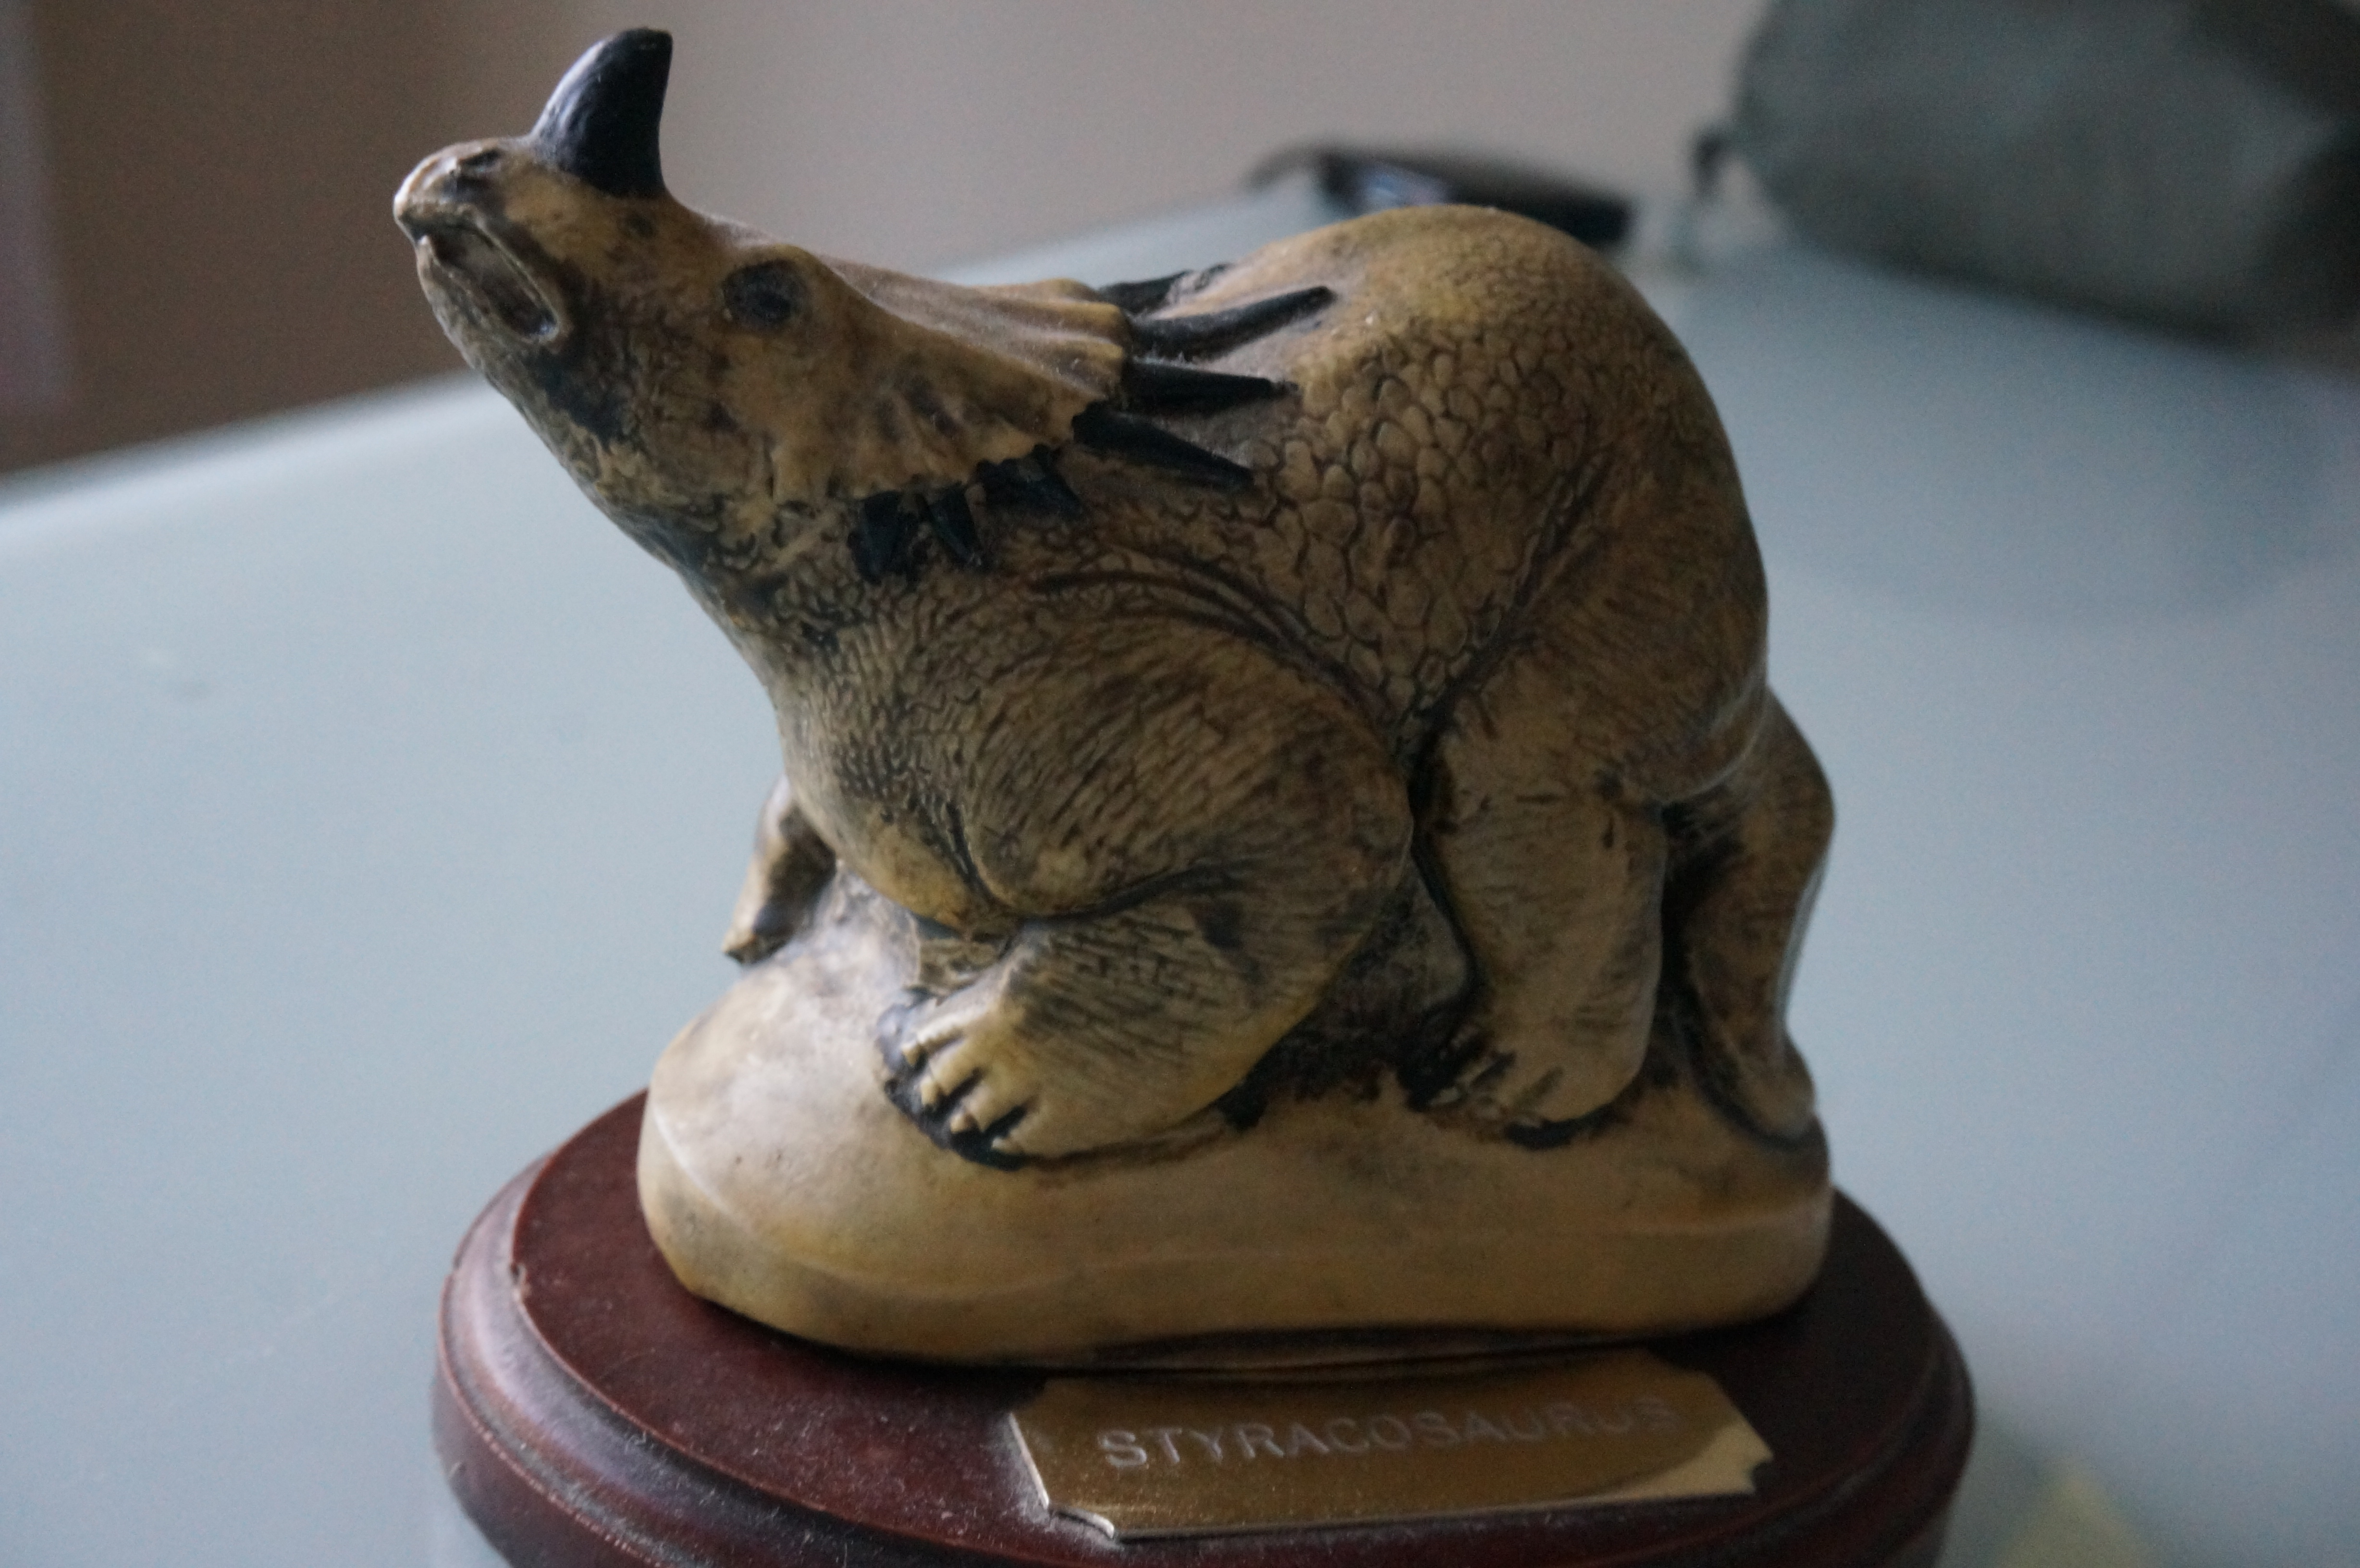
\includegraphics[width=\linewidth]{datas/dino_image.jpg}
        \caption{}
    \end{subfigure}
    \begin{subfigure}{0.47\textwidth}
        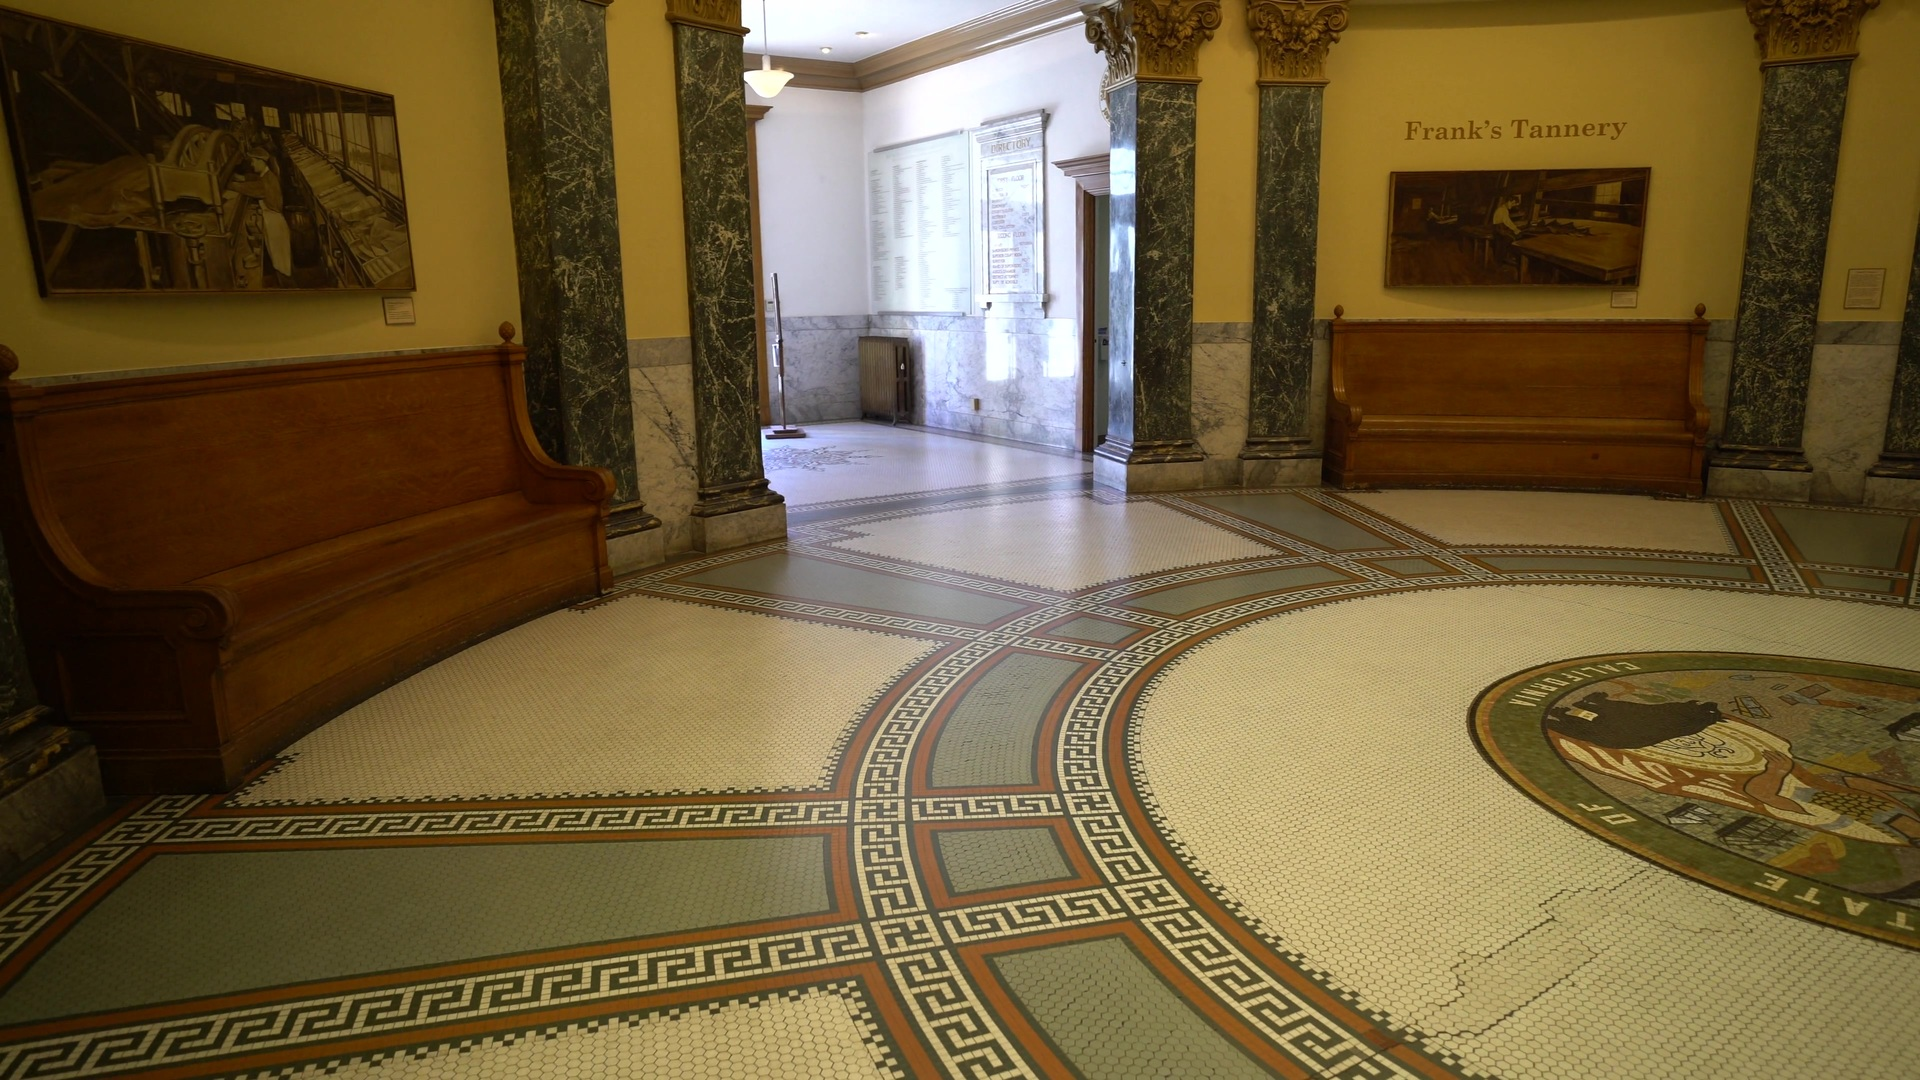
\includegraphics[width=\linewidth]{datas/museum_image.jpg}
        \caption{}
    \end{subfigure}

    \caption{Extrait du dataset \emph{Dinosaure} (a) et du dataset \emph{Museum} (b)}
    \label{fig:dataset_exemple}
\end{figure}

Explication des différents critères recherchés (C++, libre de droits, ...)

\section{Présentation des logiciels}

Présentation des différents softwares
\begin{itemize}
    \item OpenSFM
    \item VisualSFM
    \item OpenMVG + OpenMVS
    \item Alicevision Meshroom
    \item Regard3D
    \item Colmap
\end{itemize}

Affichage des résultats

\comment{Placé ici temporairement, surement déplacé en annexe après}

\begin{figure}[ht]
    \centering
    \begin{subfigure}{0.45\textwidth}
        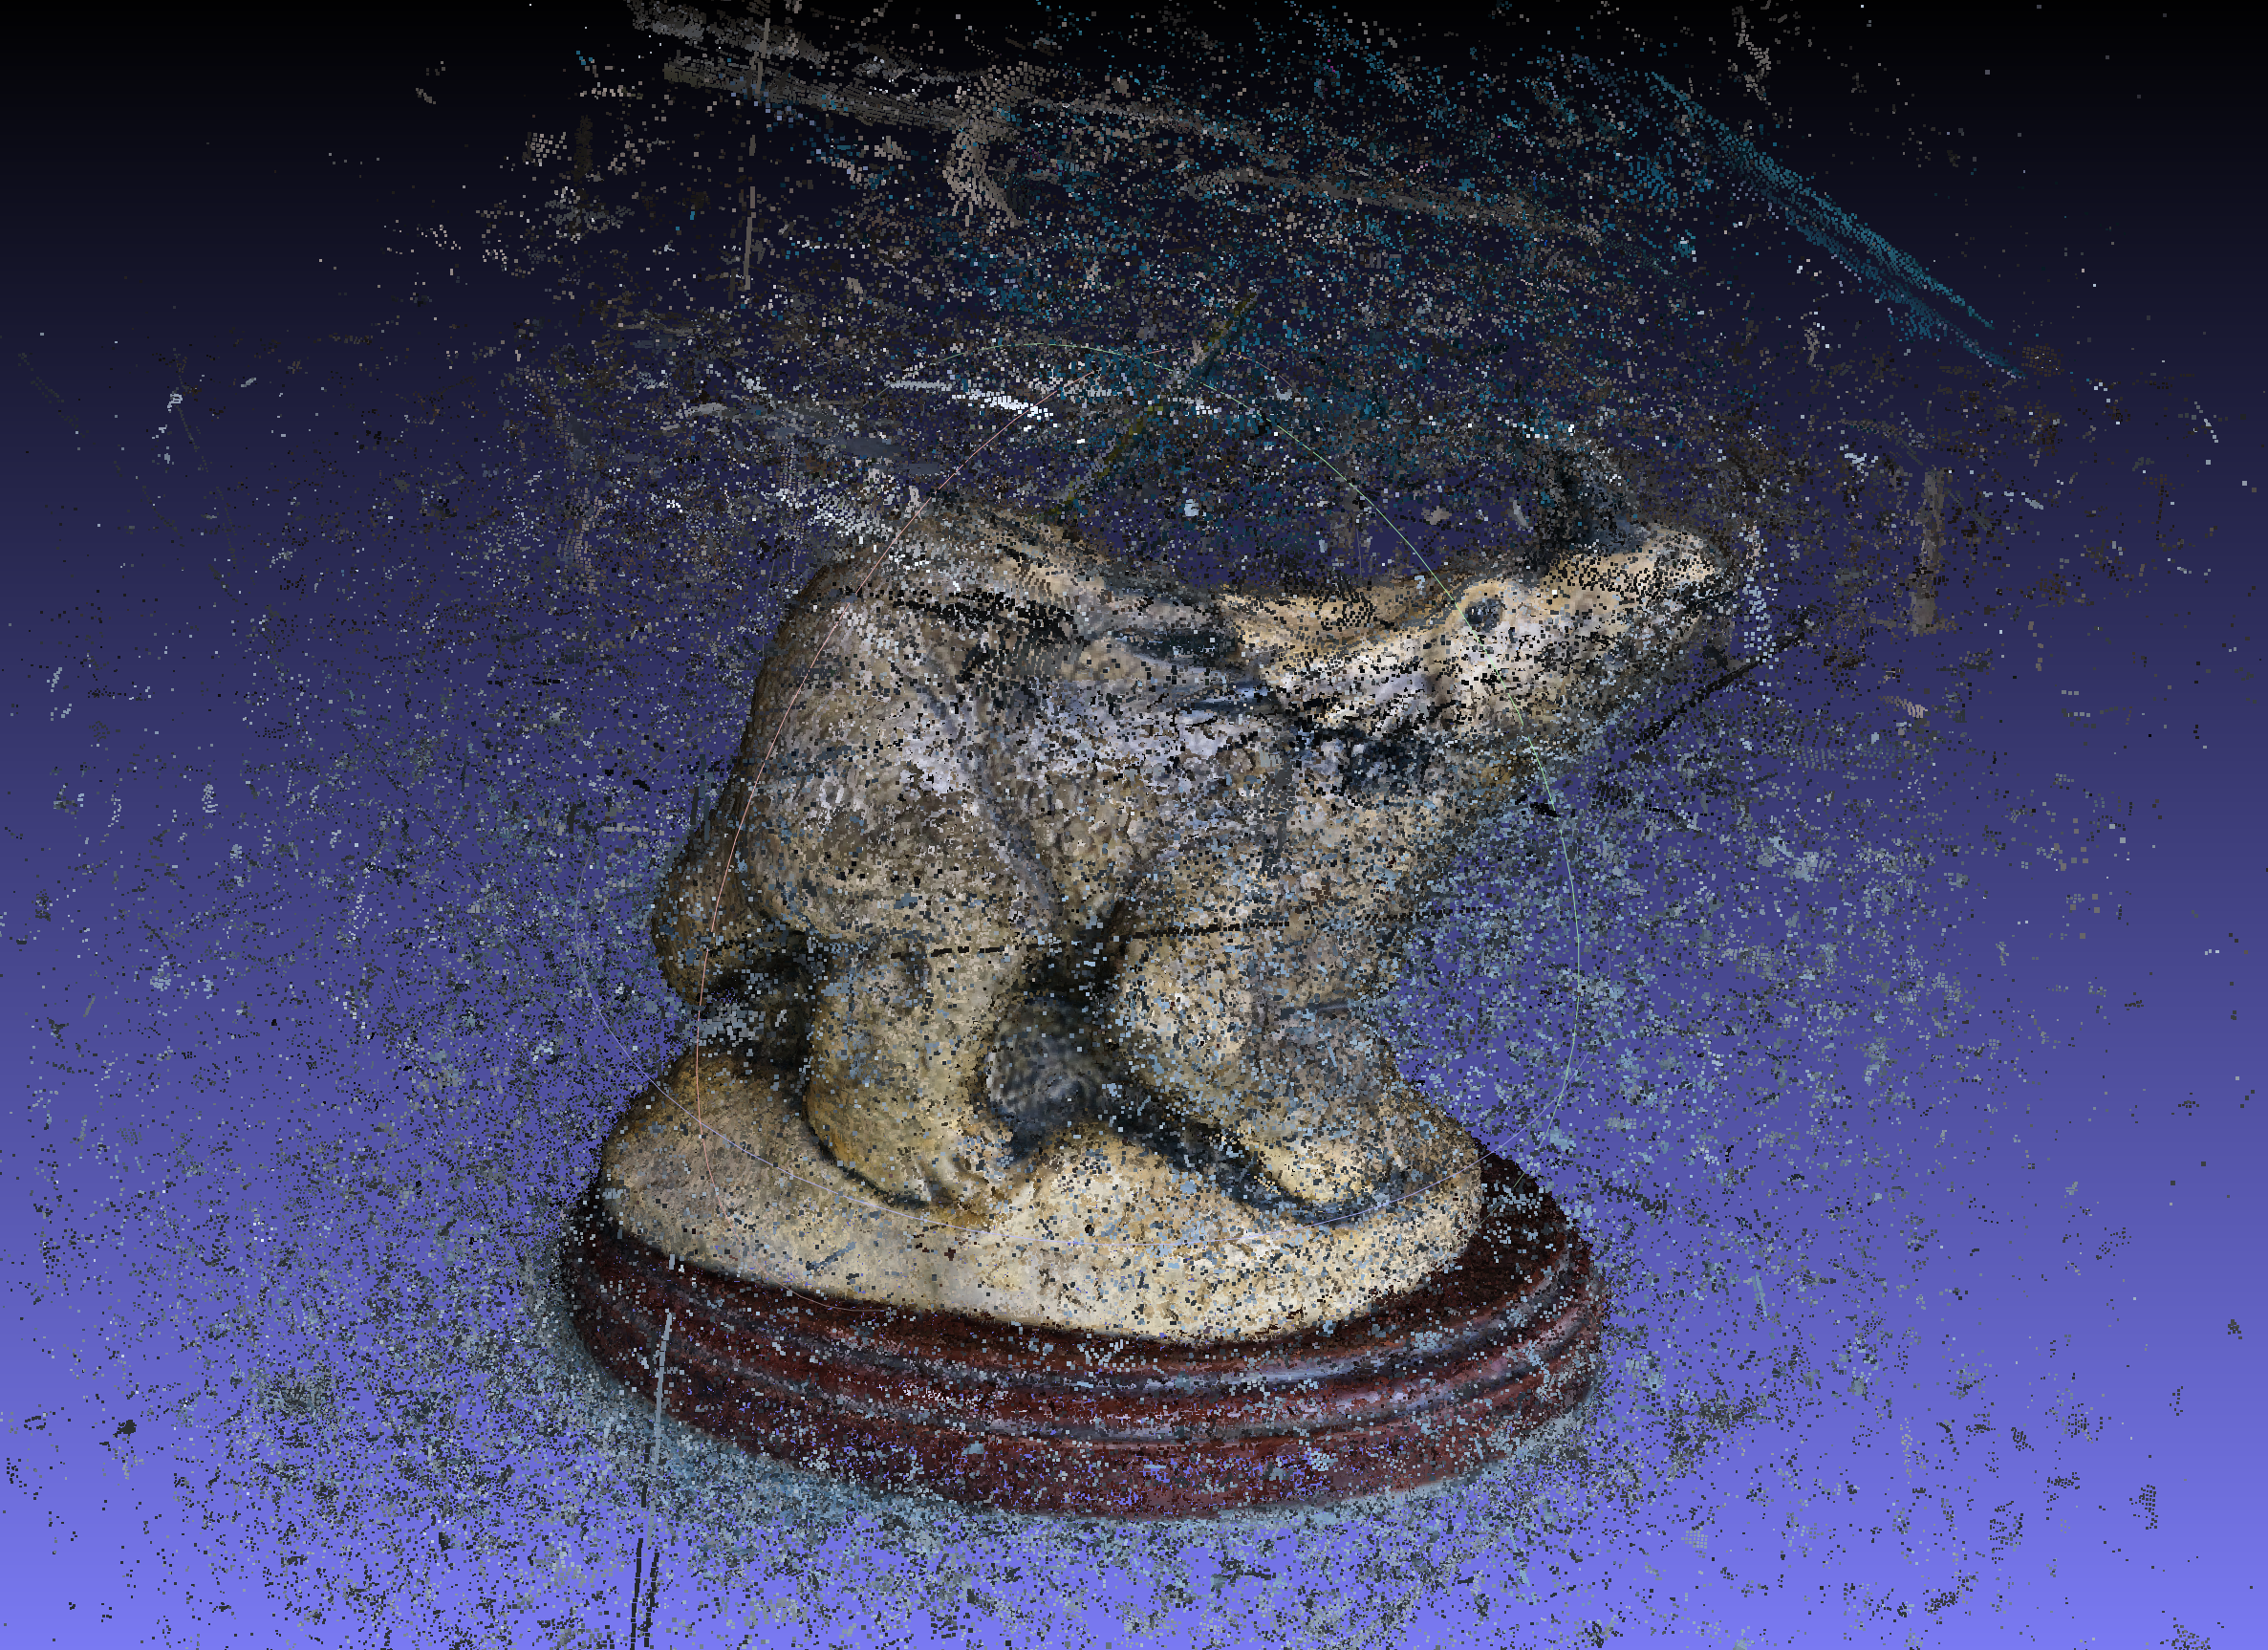
\includegraphics[width=\linewidth]{datas/state_of_the_art/opensfm_result_dino.png}
        \caption{}
    \end{subfigure}
    \begin{subfigure}{0.45\textwidth}
        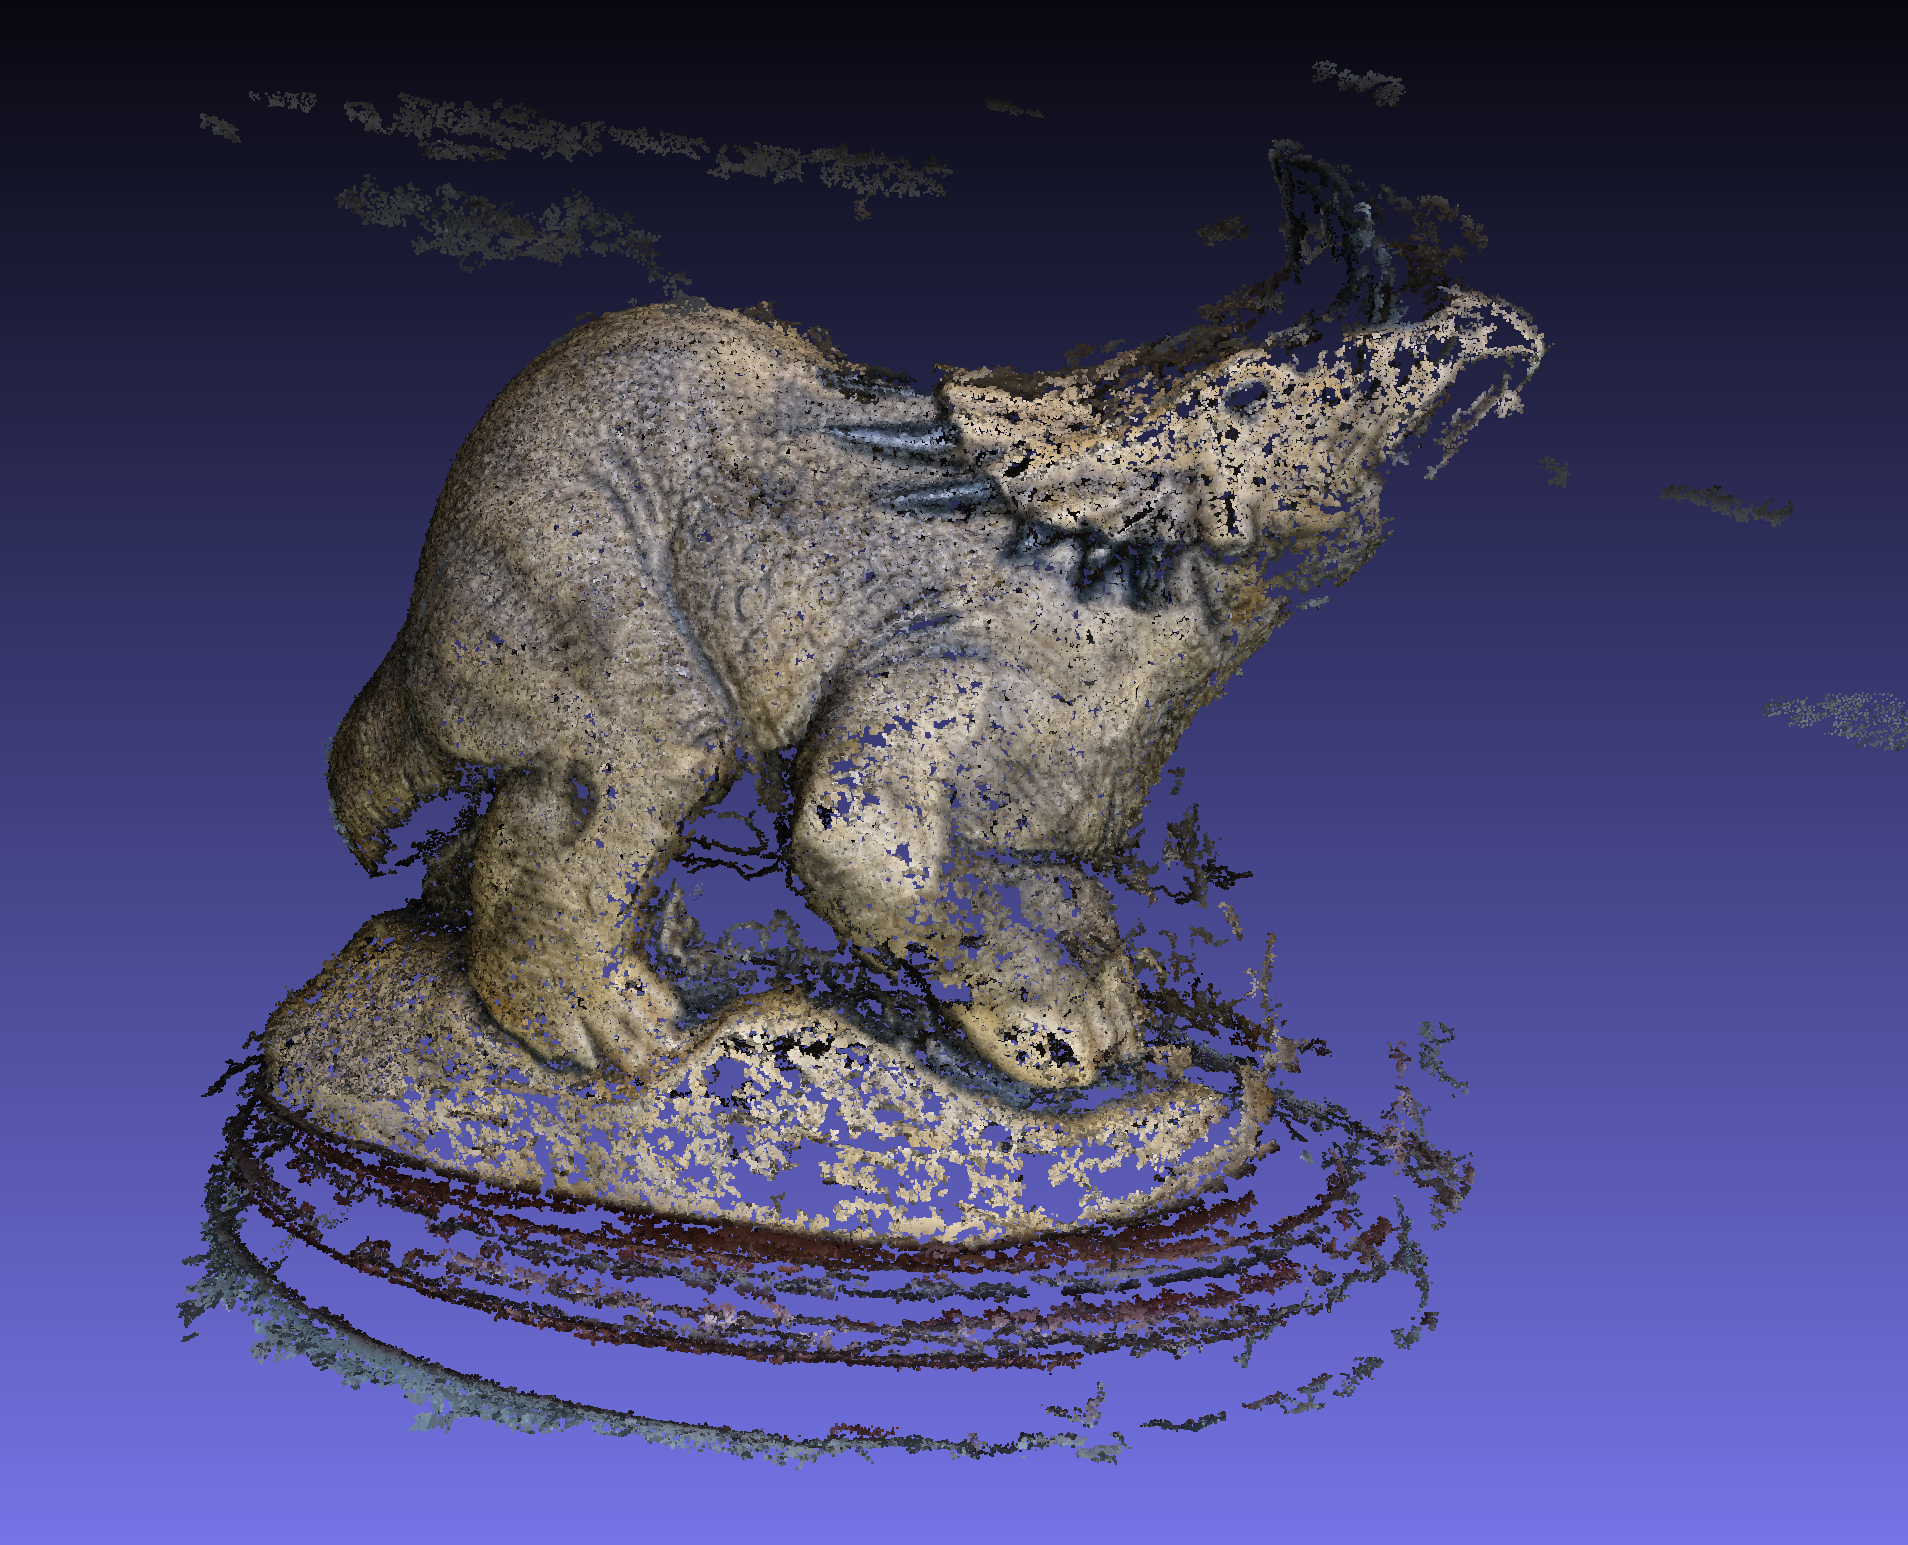
\includegraphics[width=\linewidth]{datas/state_of_the_art/visualsfm_result_dino.png}
        \caption{}
    \end{subfigure}

    \begin{subfigure}{0.45\textwidth}
        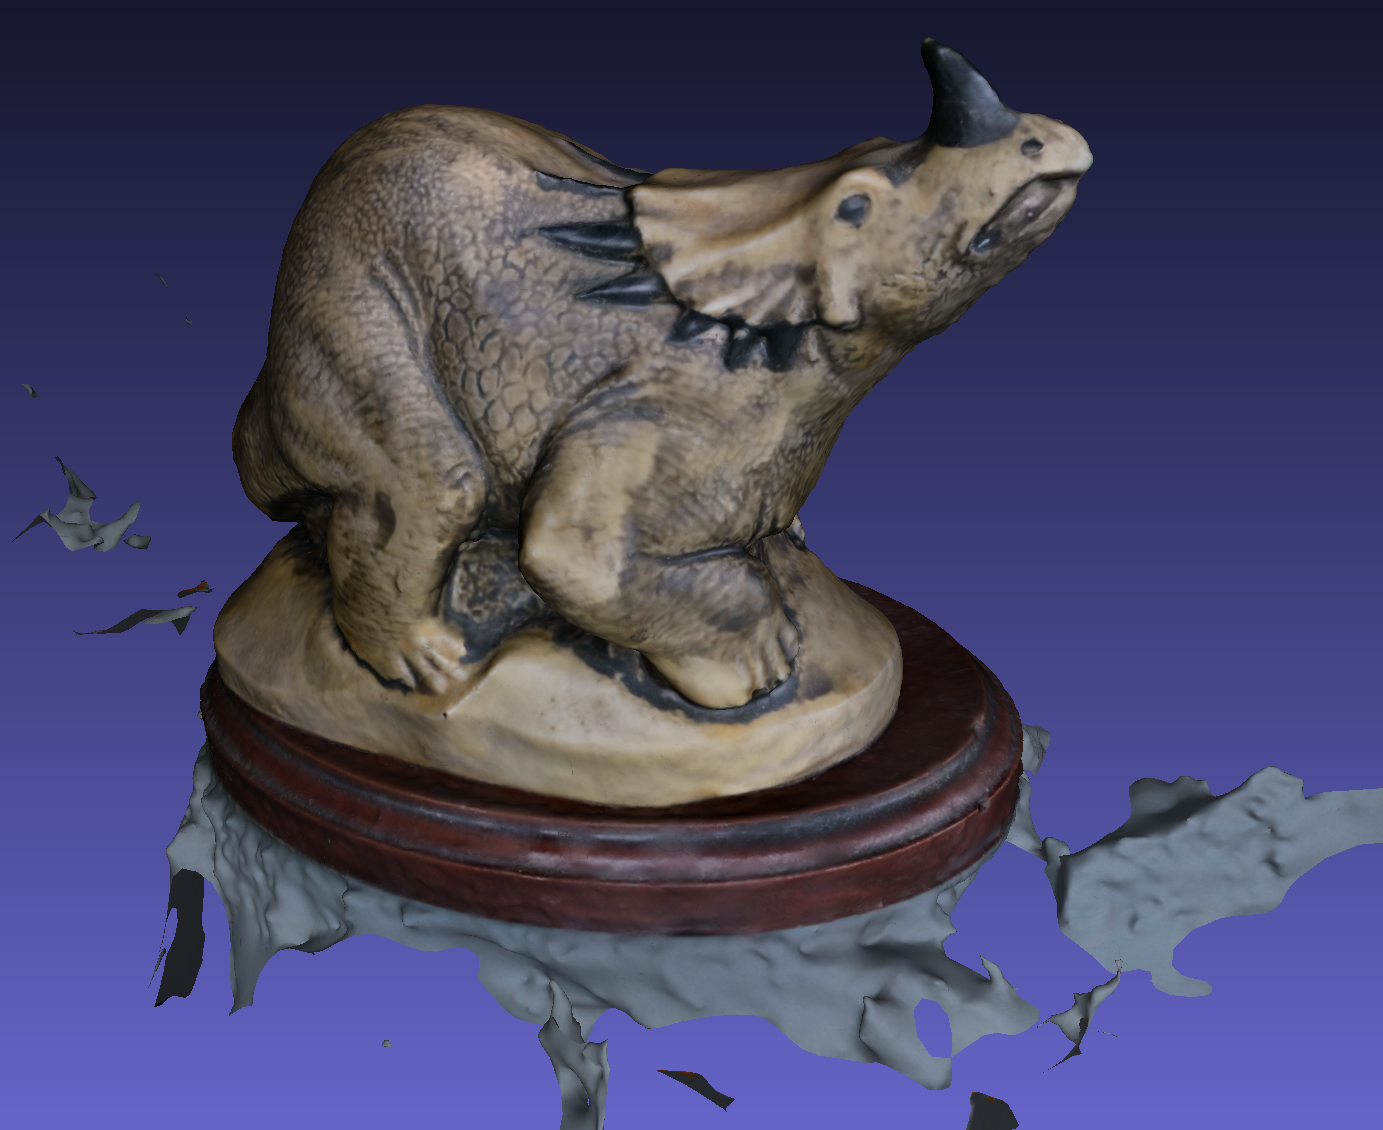
\includegraphics[width=\linewidth]{datas/state_of_the_art/openmvg_openmvs_result_dino.png}
        \caption{}
    \end{subfigure}
    \begin{subfigure}{0.45\textwidth}
        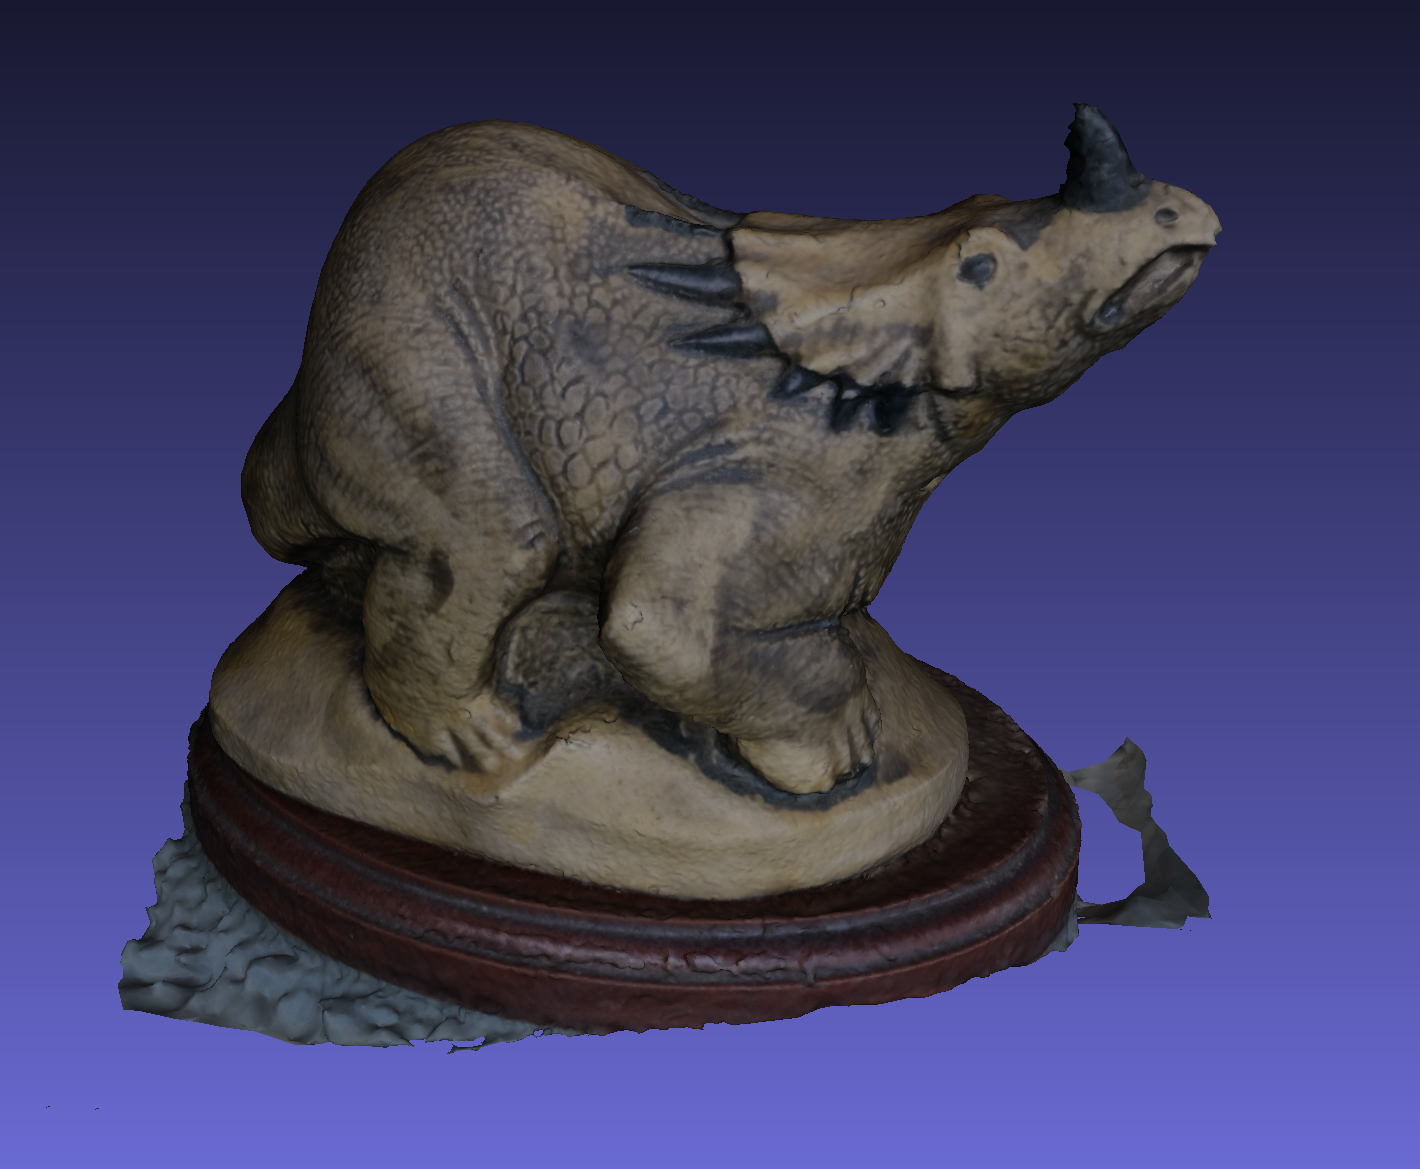
\includegraphics[width=\linewidth]{datas/state_of_the_art/meshroom_result_dino.png}
        \caption{}
    \end{subfigure}

    \begin{subfigure}{0.45\textwidth}
        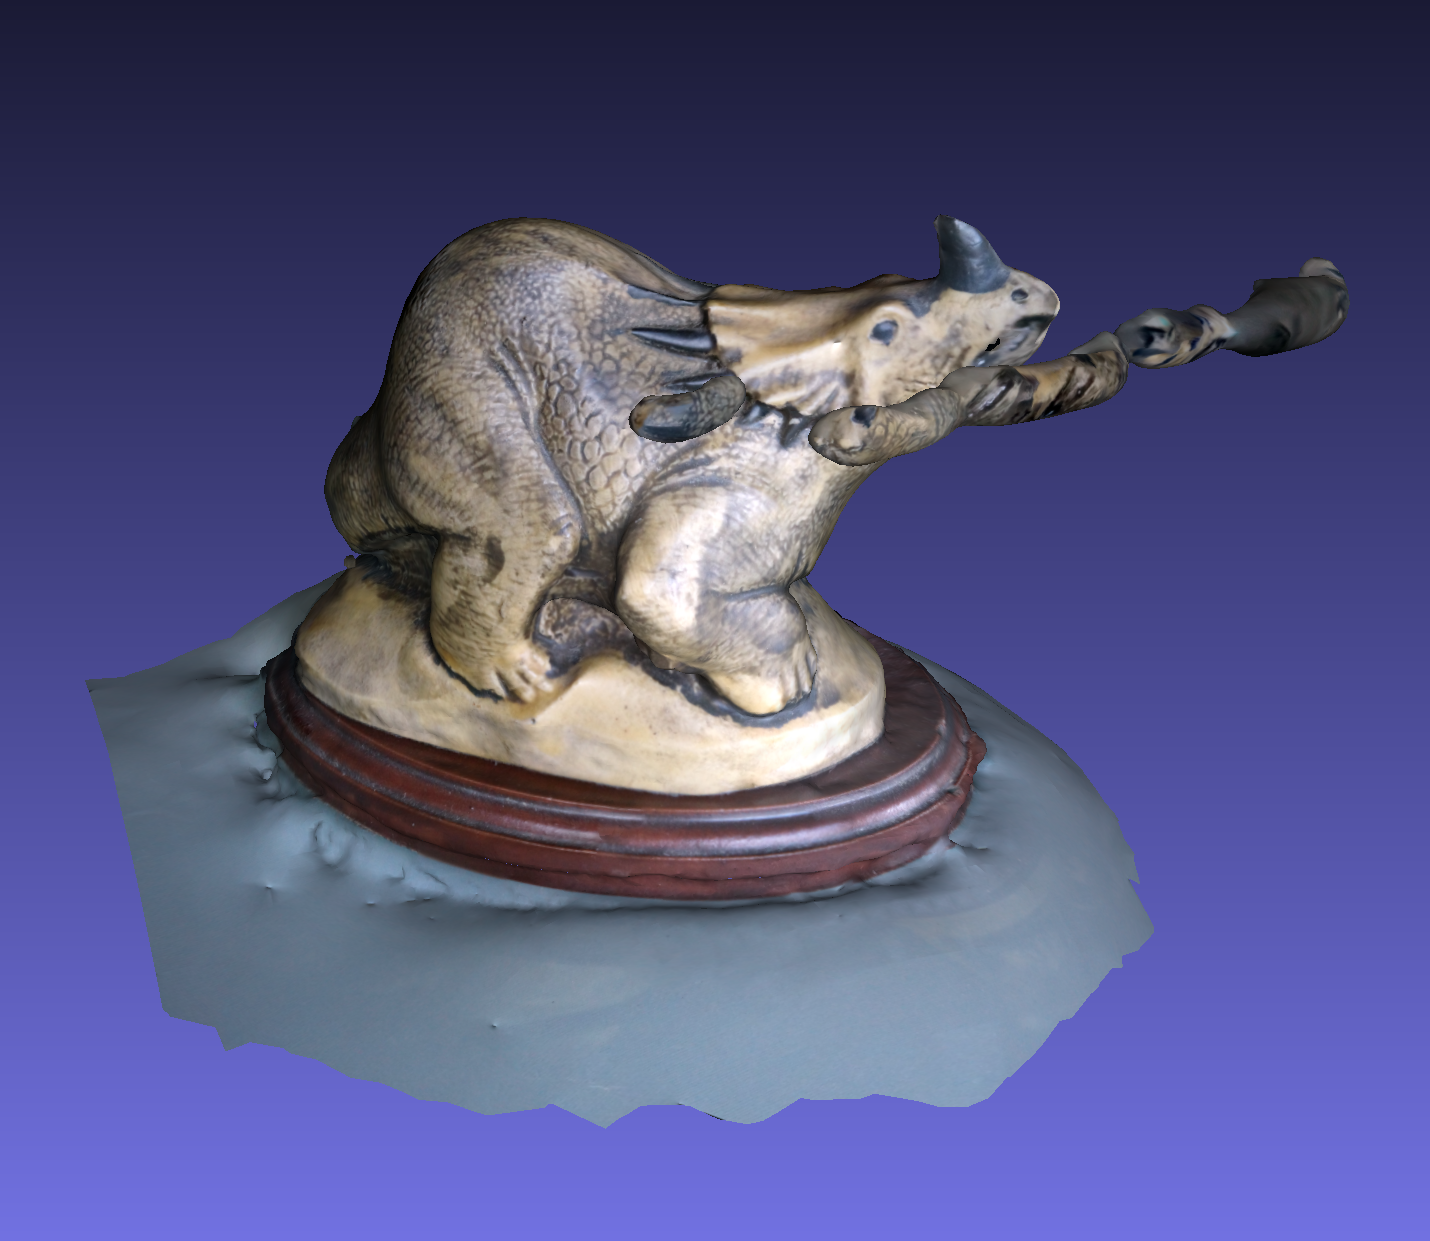
\includegraphics[width=\linewidth]{datas/state_of_the_art/regard3d_result_dino.png}
        \caption{}
    \end{subfigure}
    \begin{subfigure}{0.45\textwidth}
        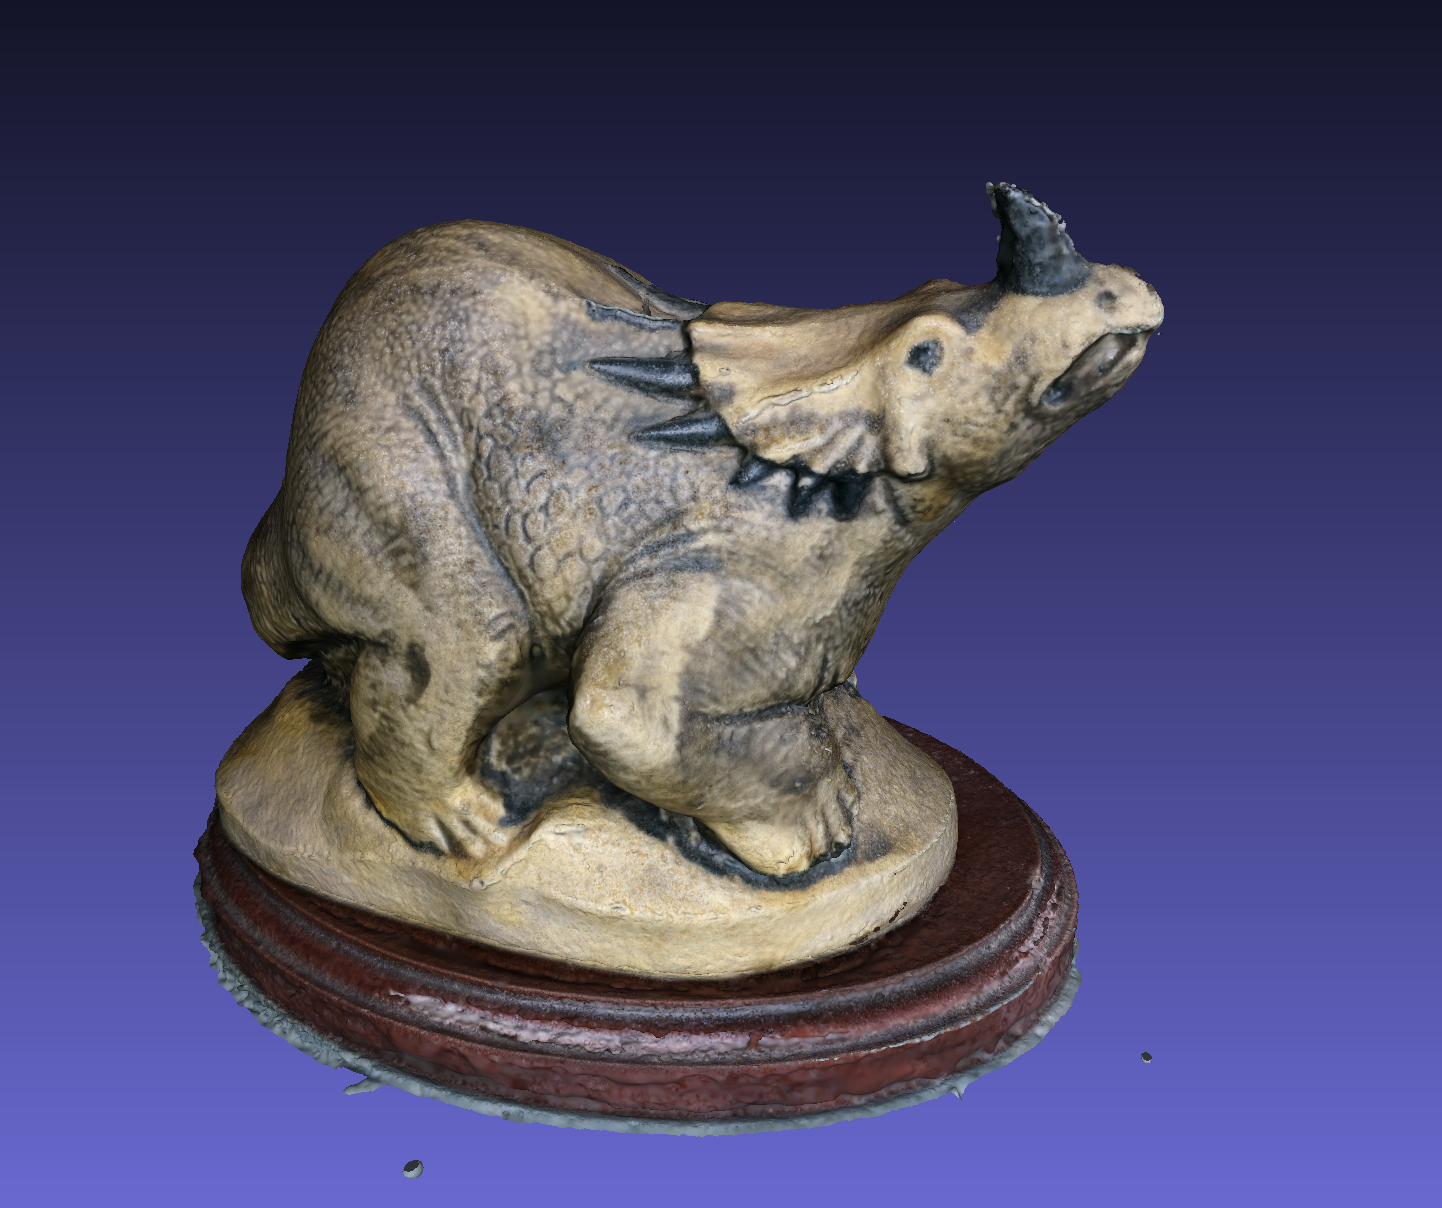
\includegraphics[width=\linewidth]{datas/state_of_the_art/colmap_result_dino.png}
        \caption{}
    \end{subfigure}

    \caption{Résultats de l'état de l'art avec le dataset Dinosaure : (a)OpenSFM, (b)VisualSFM, (c)OpenMVG+OpenMVS, (d)Alicevision Meshroom, (e)Regard3D, (f)Colmap}
    \label{fig:result_sota}
\end{figure}

\section{Choix final}

Explication du choix final

Transition vers la partie suivante

% \chapter{Conclusion}

Bilan travail accompli

Bilan sur le futur du projet

Bilan personnel

\nocite{*}
\bibliography{bibliographie}
\bibliographystyle{plain}

% \appendix
\addcontentsline{toc}{chapter}{Annexes}
\chapter*{Annexes}

\begin{figure}[ht]
    \centering
    \begin{subfigure}{0.37\textwidth}
        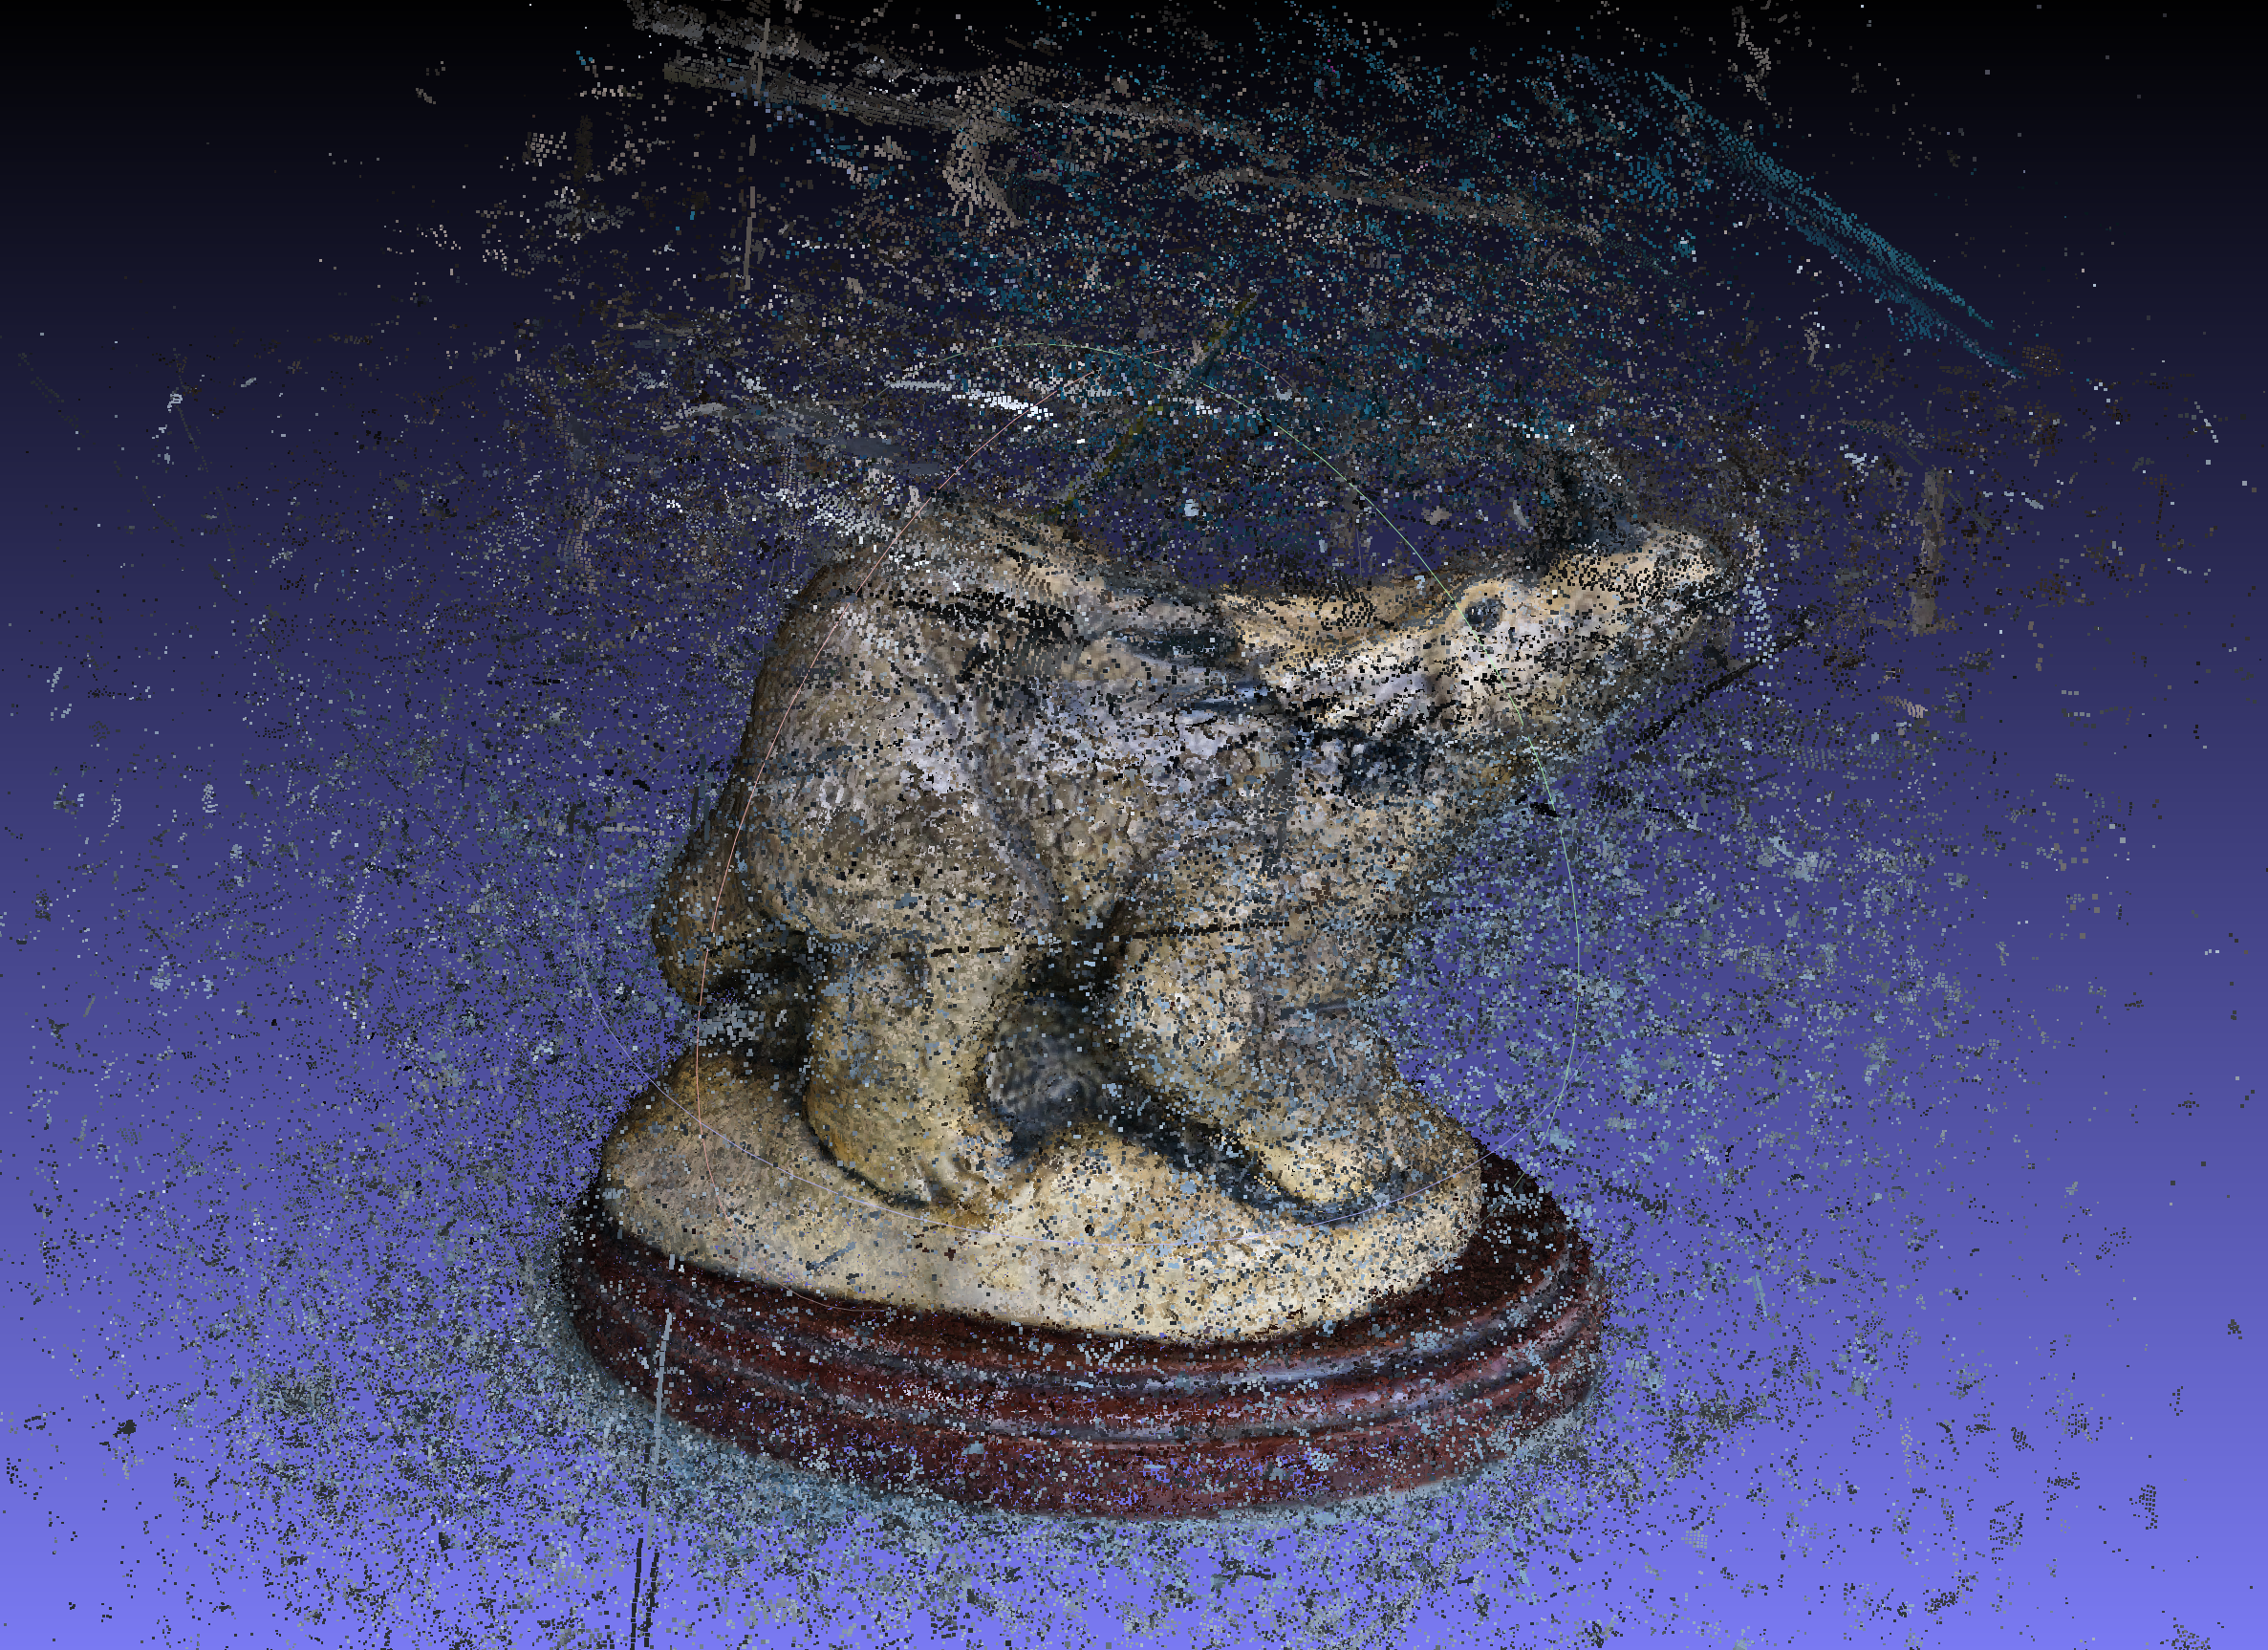
\includegraphics[width=\linewidth]{datas/state_of_the_art/opensfm_result_dino.png}
        \caption{}
    \end{subfigure}
    \begin{subfigure}{0.37\textwidth}
        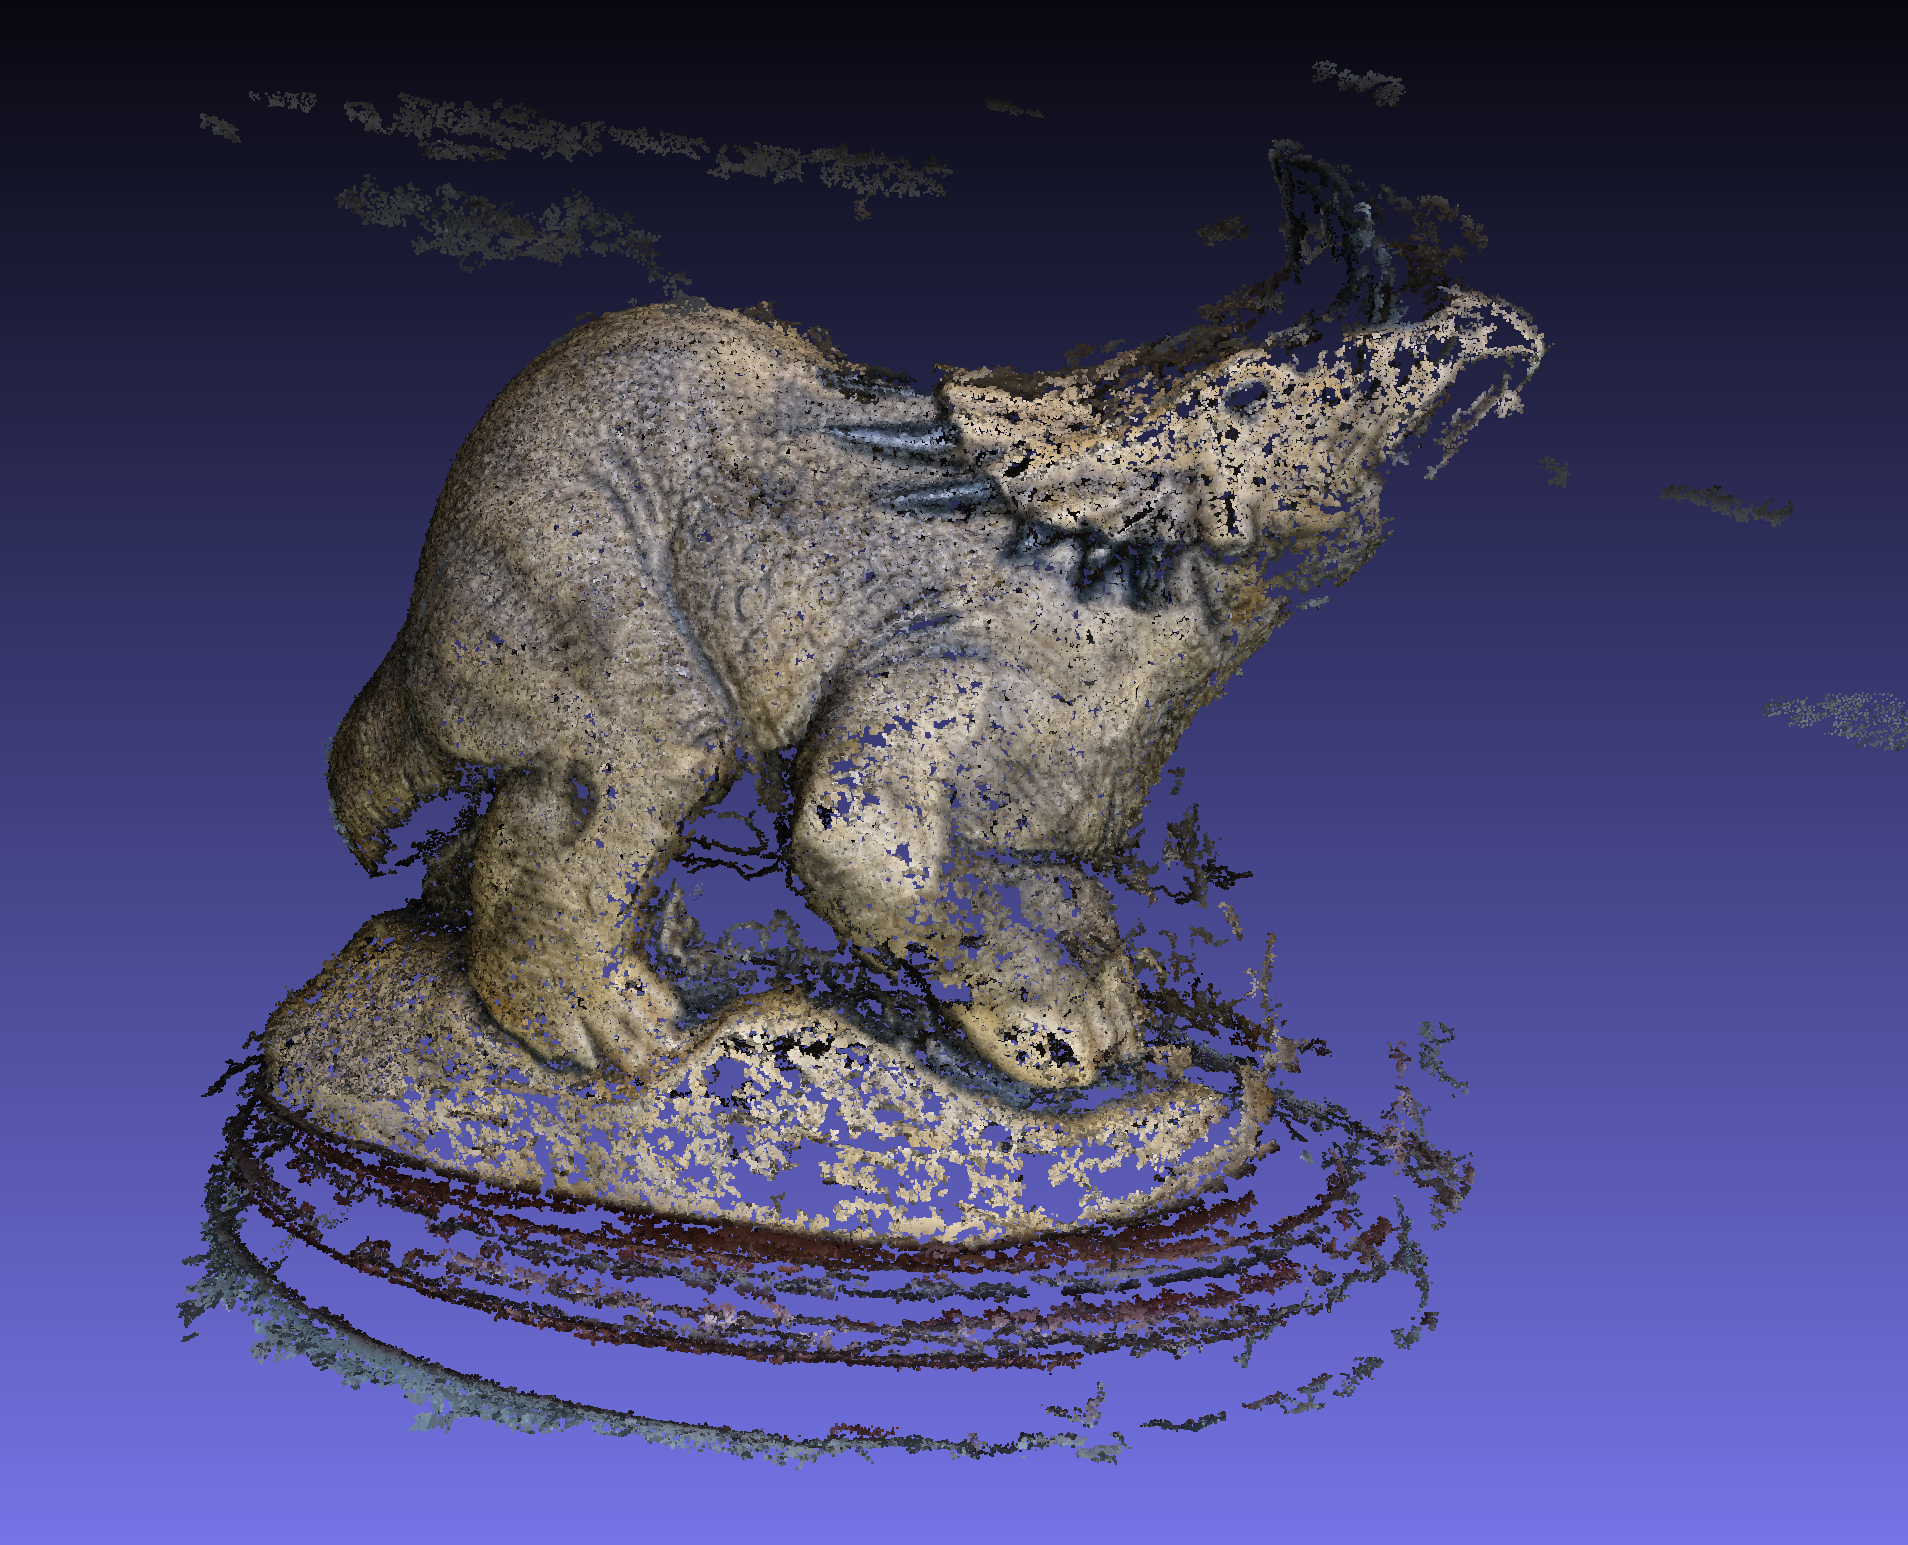
\includegraphics[width=\linewidth]{datas/state_of_the_art/visualsfm_result_dino.png}
        \caption{}
    \end{subfigure}

    \begin{subfigure}{0.37\textwidth}
        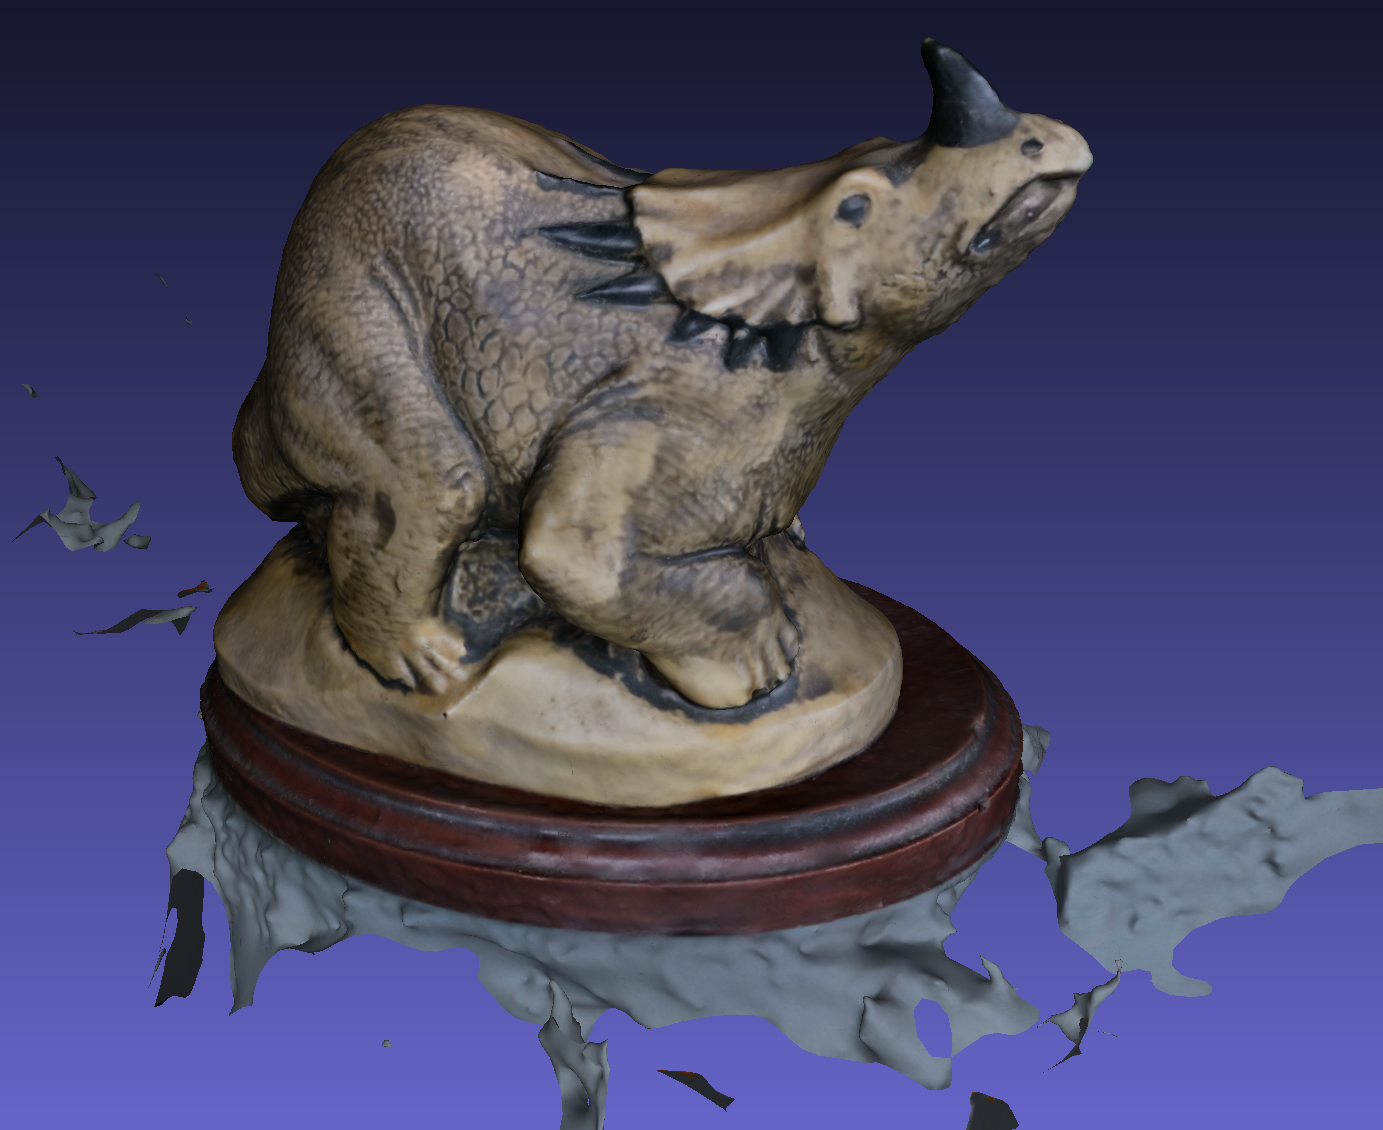
\includegraphics[width=\linewidth]{datas/state_of_the_art/openmvg_openmvs_result_dino.png}
        \caption{}
    \end{subfigure}
    \begin{subfigure}{0.37\textwidth}
        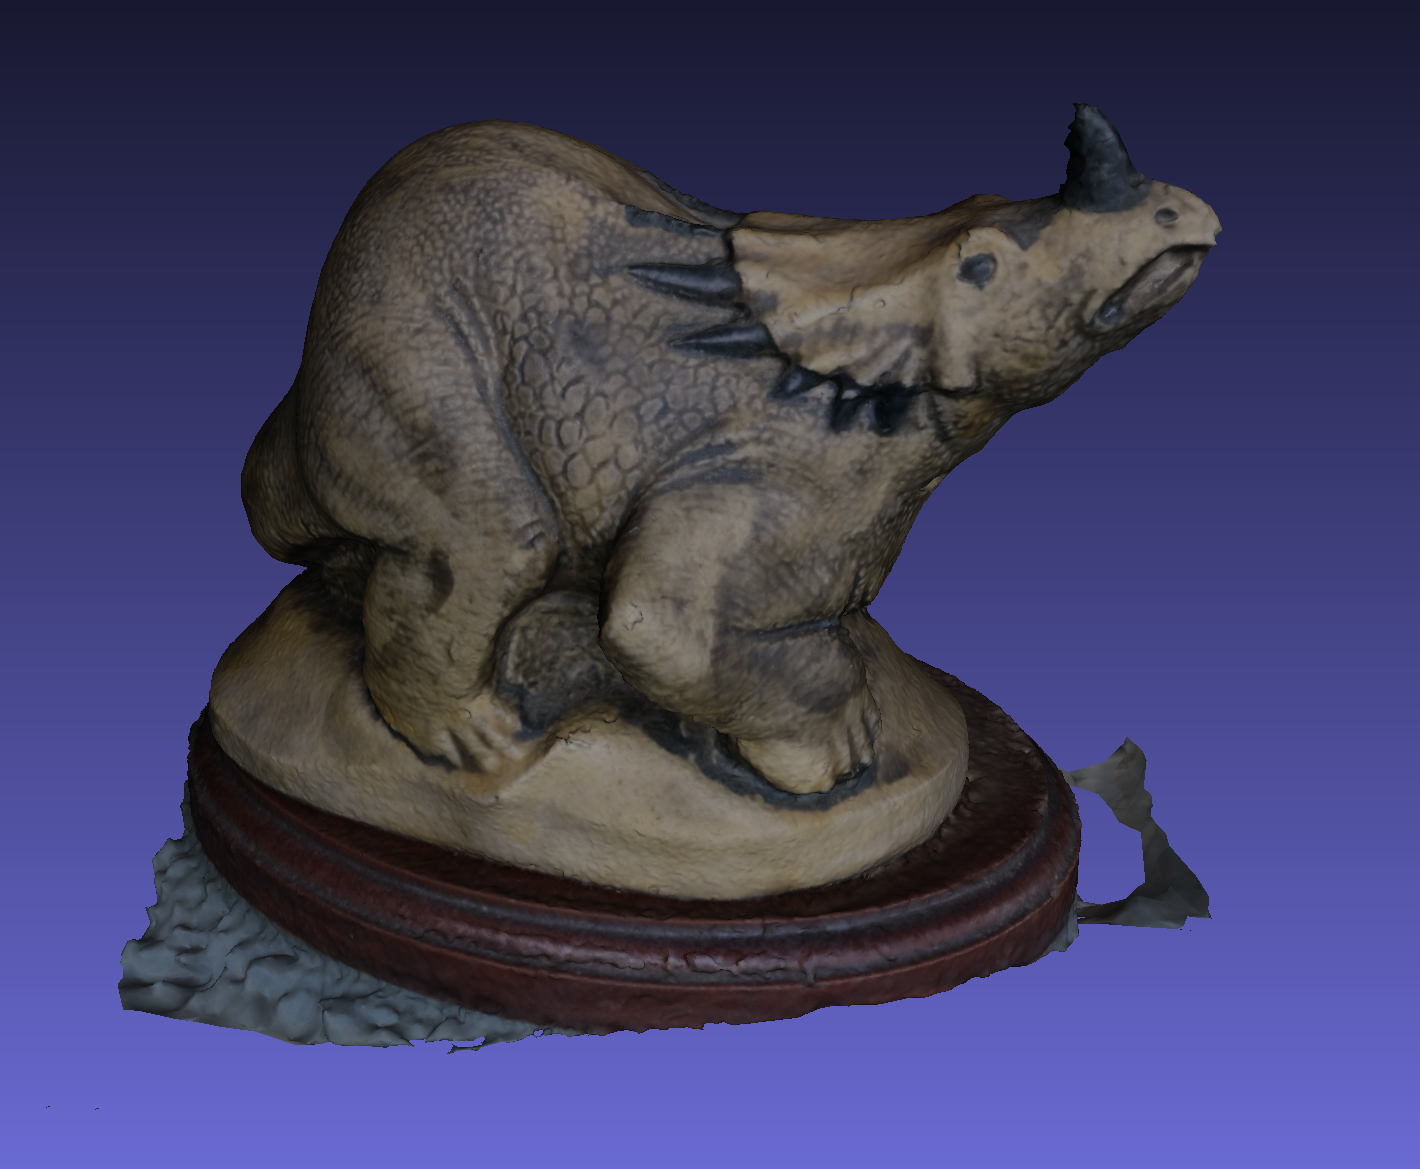
\includegraphics[width=\linewidth]{datas/state_of_the_art/meshroom_result_dino.png}
        \caption{}
    \end{subfigure}

    \begin{subfigure}{0.37\textwidth}
        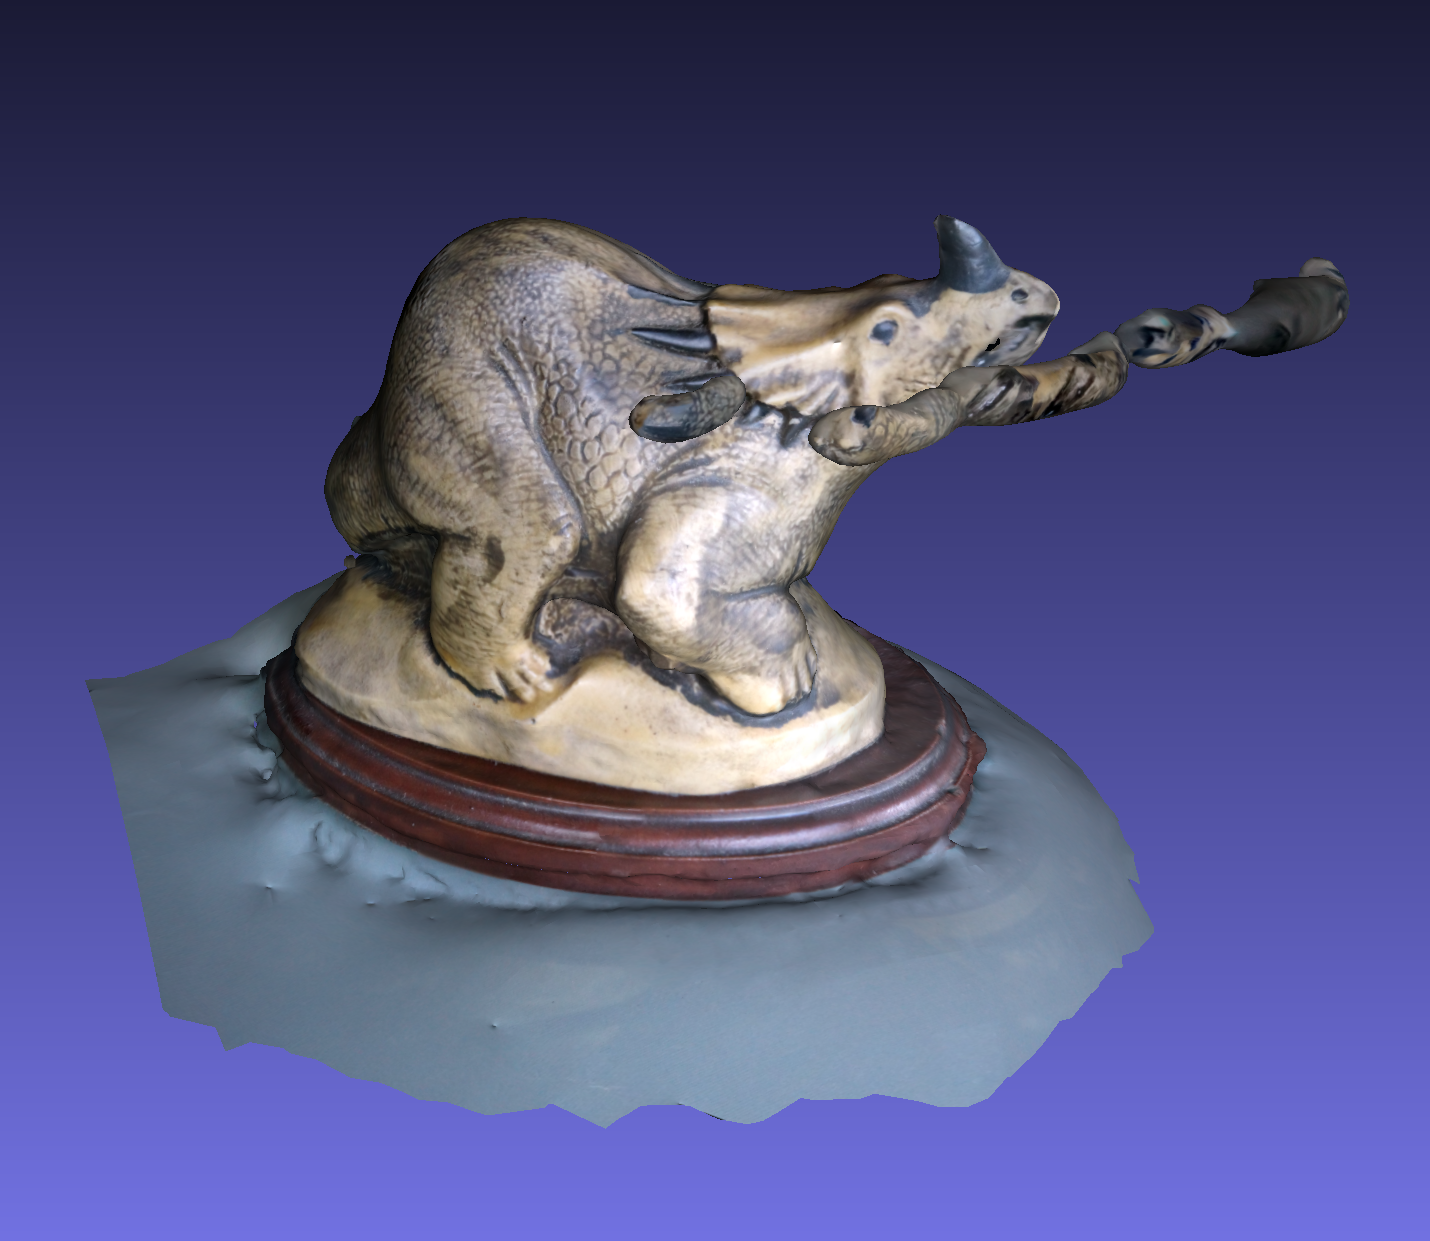
\includegraphics[width=\linewidth]{datas/state_of_the_art/regard3d_result_dino.png}
        \caption{}
    \end{subfigure}
    \begin{subfigure}{0.37\textwidth}
        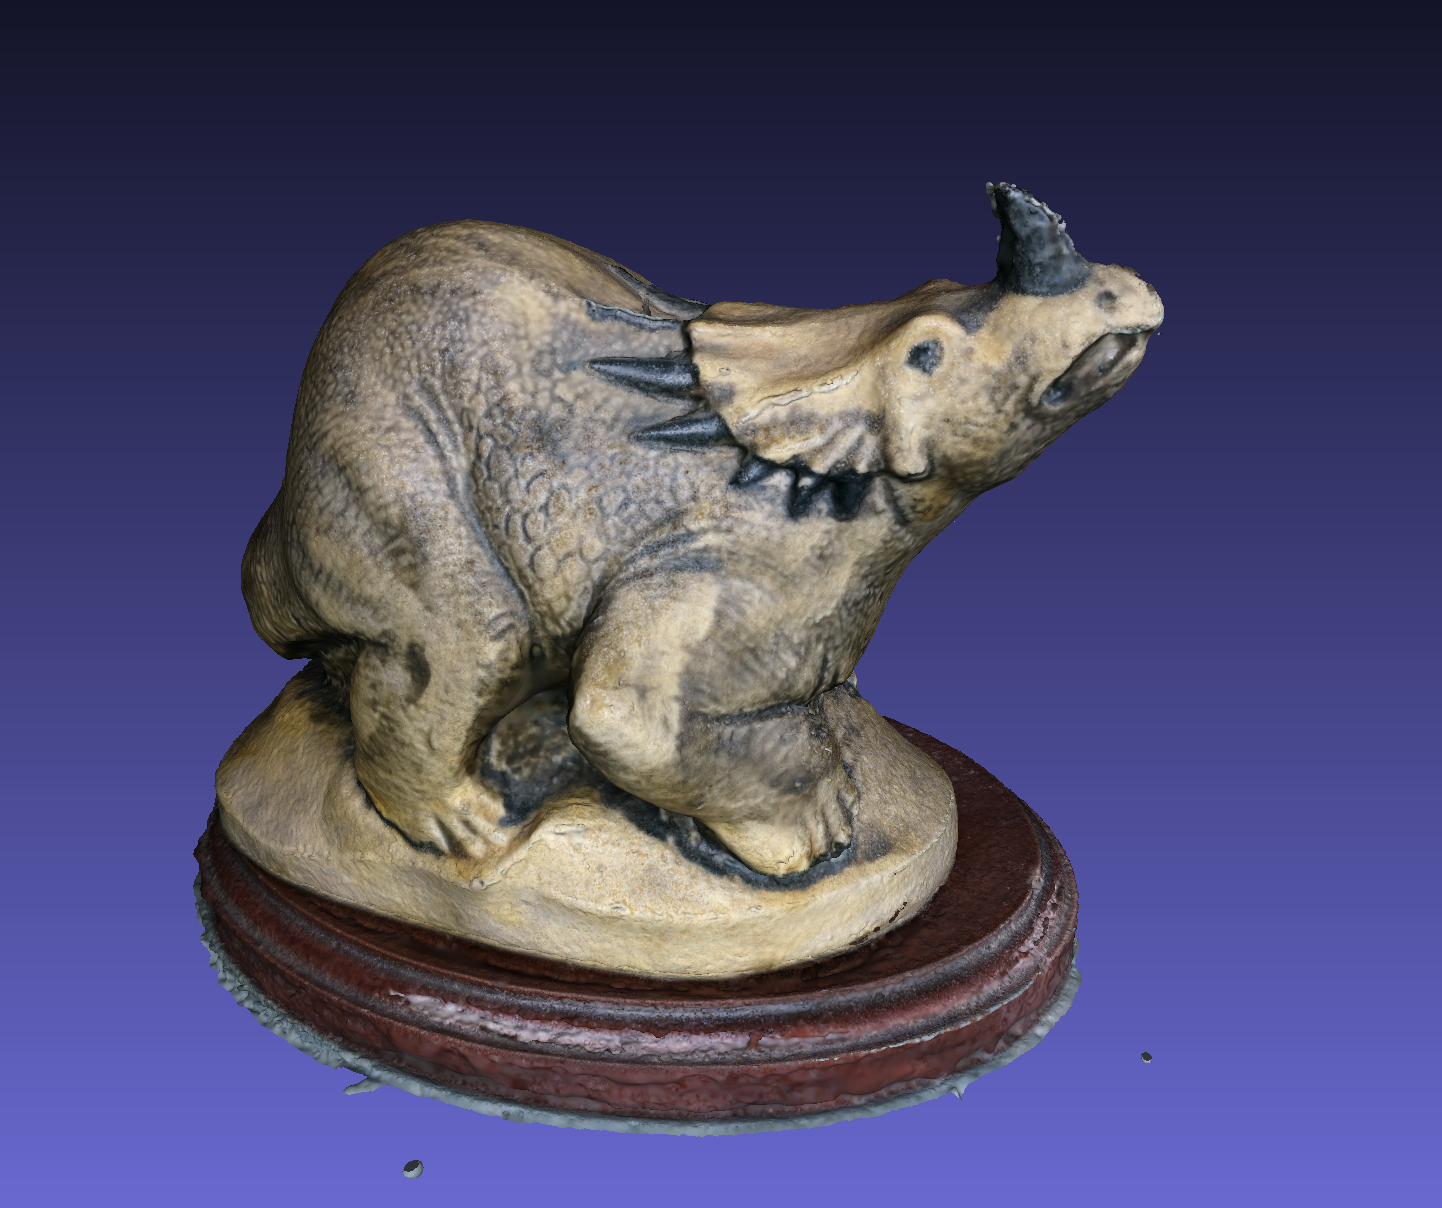
\includegraphics[width=\linewidth]{datas/state_of_the_art/colmap_result_dino.png}
        \caption{}
    \end{subfigure}

    \caption{Résultats de l'état de l'art avec le dataset Dinosaure : (a)OpenSFM, (b)VisualSFM, (c)OpenMVG+OpenMVS, (d)Alicevision Meshroom, (e)Regard3D, (f)Colmap}
    \label{fig:results_etat_art}
\end{figure}

\begin{figure}[ht]
    \centering
    \begin{subfigure}{0.7\textwidth}
        \includegraphics[width=\linewidth]{datas/helper/test_keyframe_dino.png}
    \end{subfigure}

    \begin{subfigure}{0.7\textwidth}
        \includegraphics[width=\linewidth]{datas/helper/test_descriptors_dino.png}
    \end{subfigure}

    \begin{subfigure}{0.7\textwidth}
        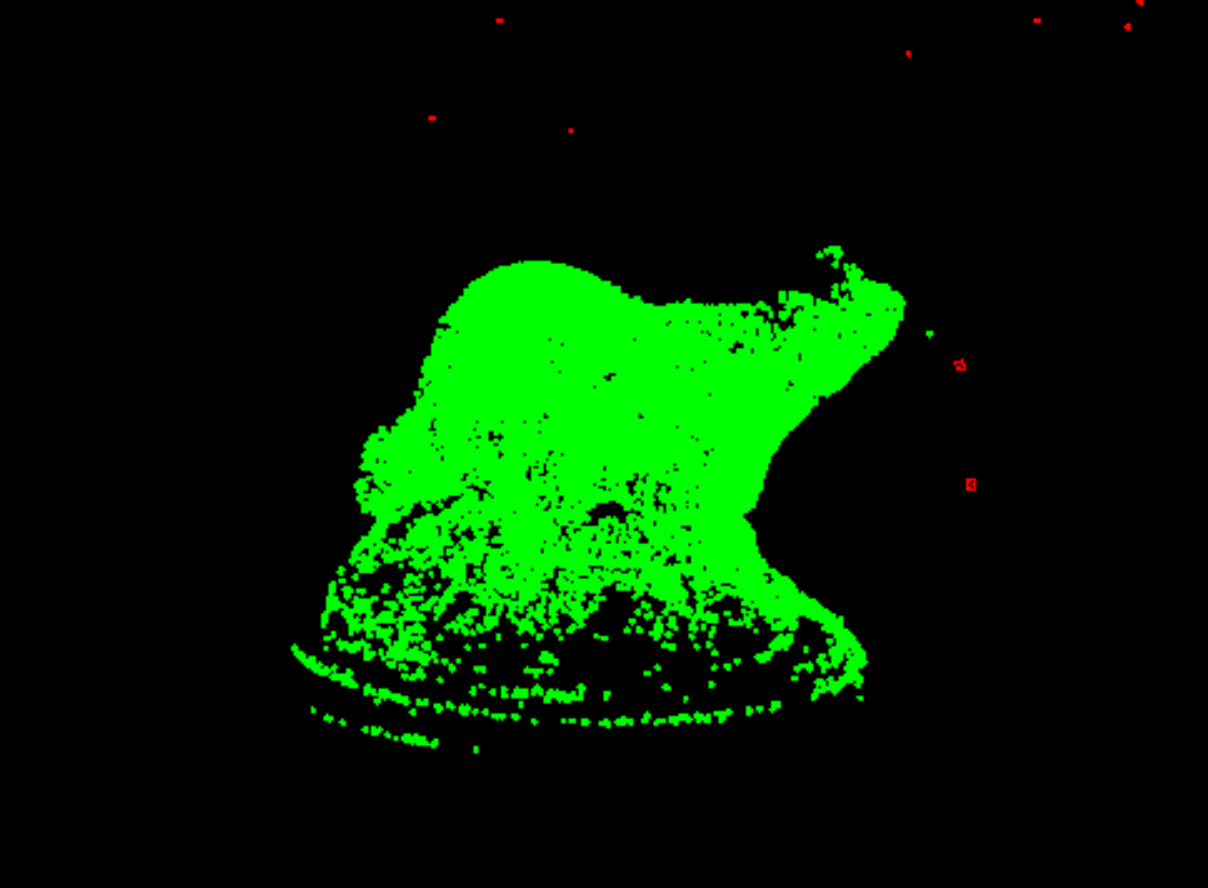
\includegraphics[width=\linewidth]{datas/helper/test_pointcloud_dino.png}
    \end{subfigure}

    \caption{Résultats des tests pour le dataset Dinosaure}
    \label{fig:test_dino}
\end{figure}

\begin{figure}[ht]
    \centering
    \begin{subfigure}{0.7\textwidth}
        \includegraphics[width=\linewidth]{datas/helper/test_keyframe_museum.png}
    \end{subfigure}

    \begin{subfigure}{0.7\textwidth}
        \includegraphics[width=\linewidth]{datas/helper/test_descriptors_museum.png}
    \end{subfigure}

    \begin{subfigure}{0.7\textwidth}
        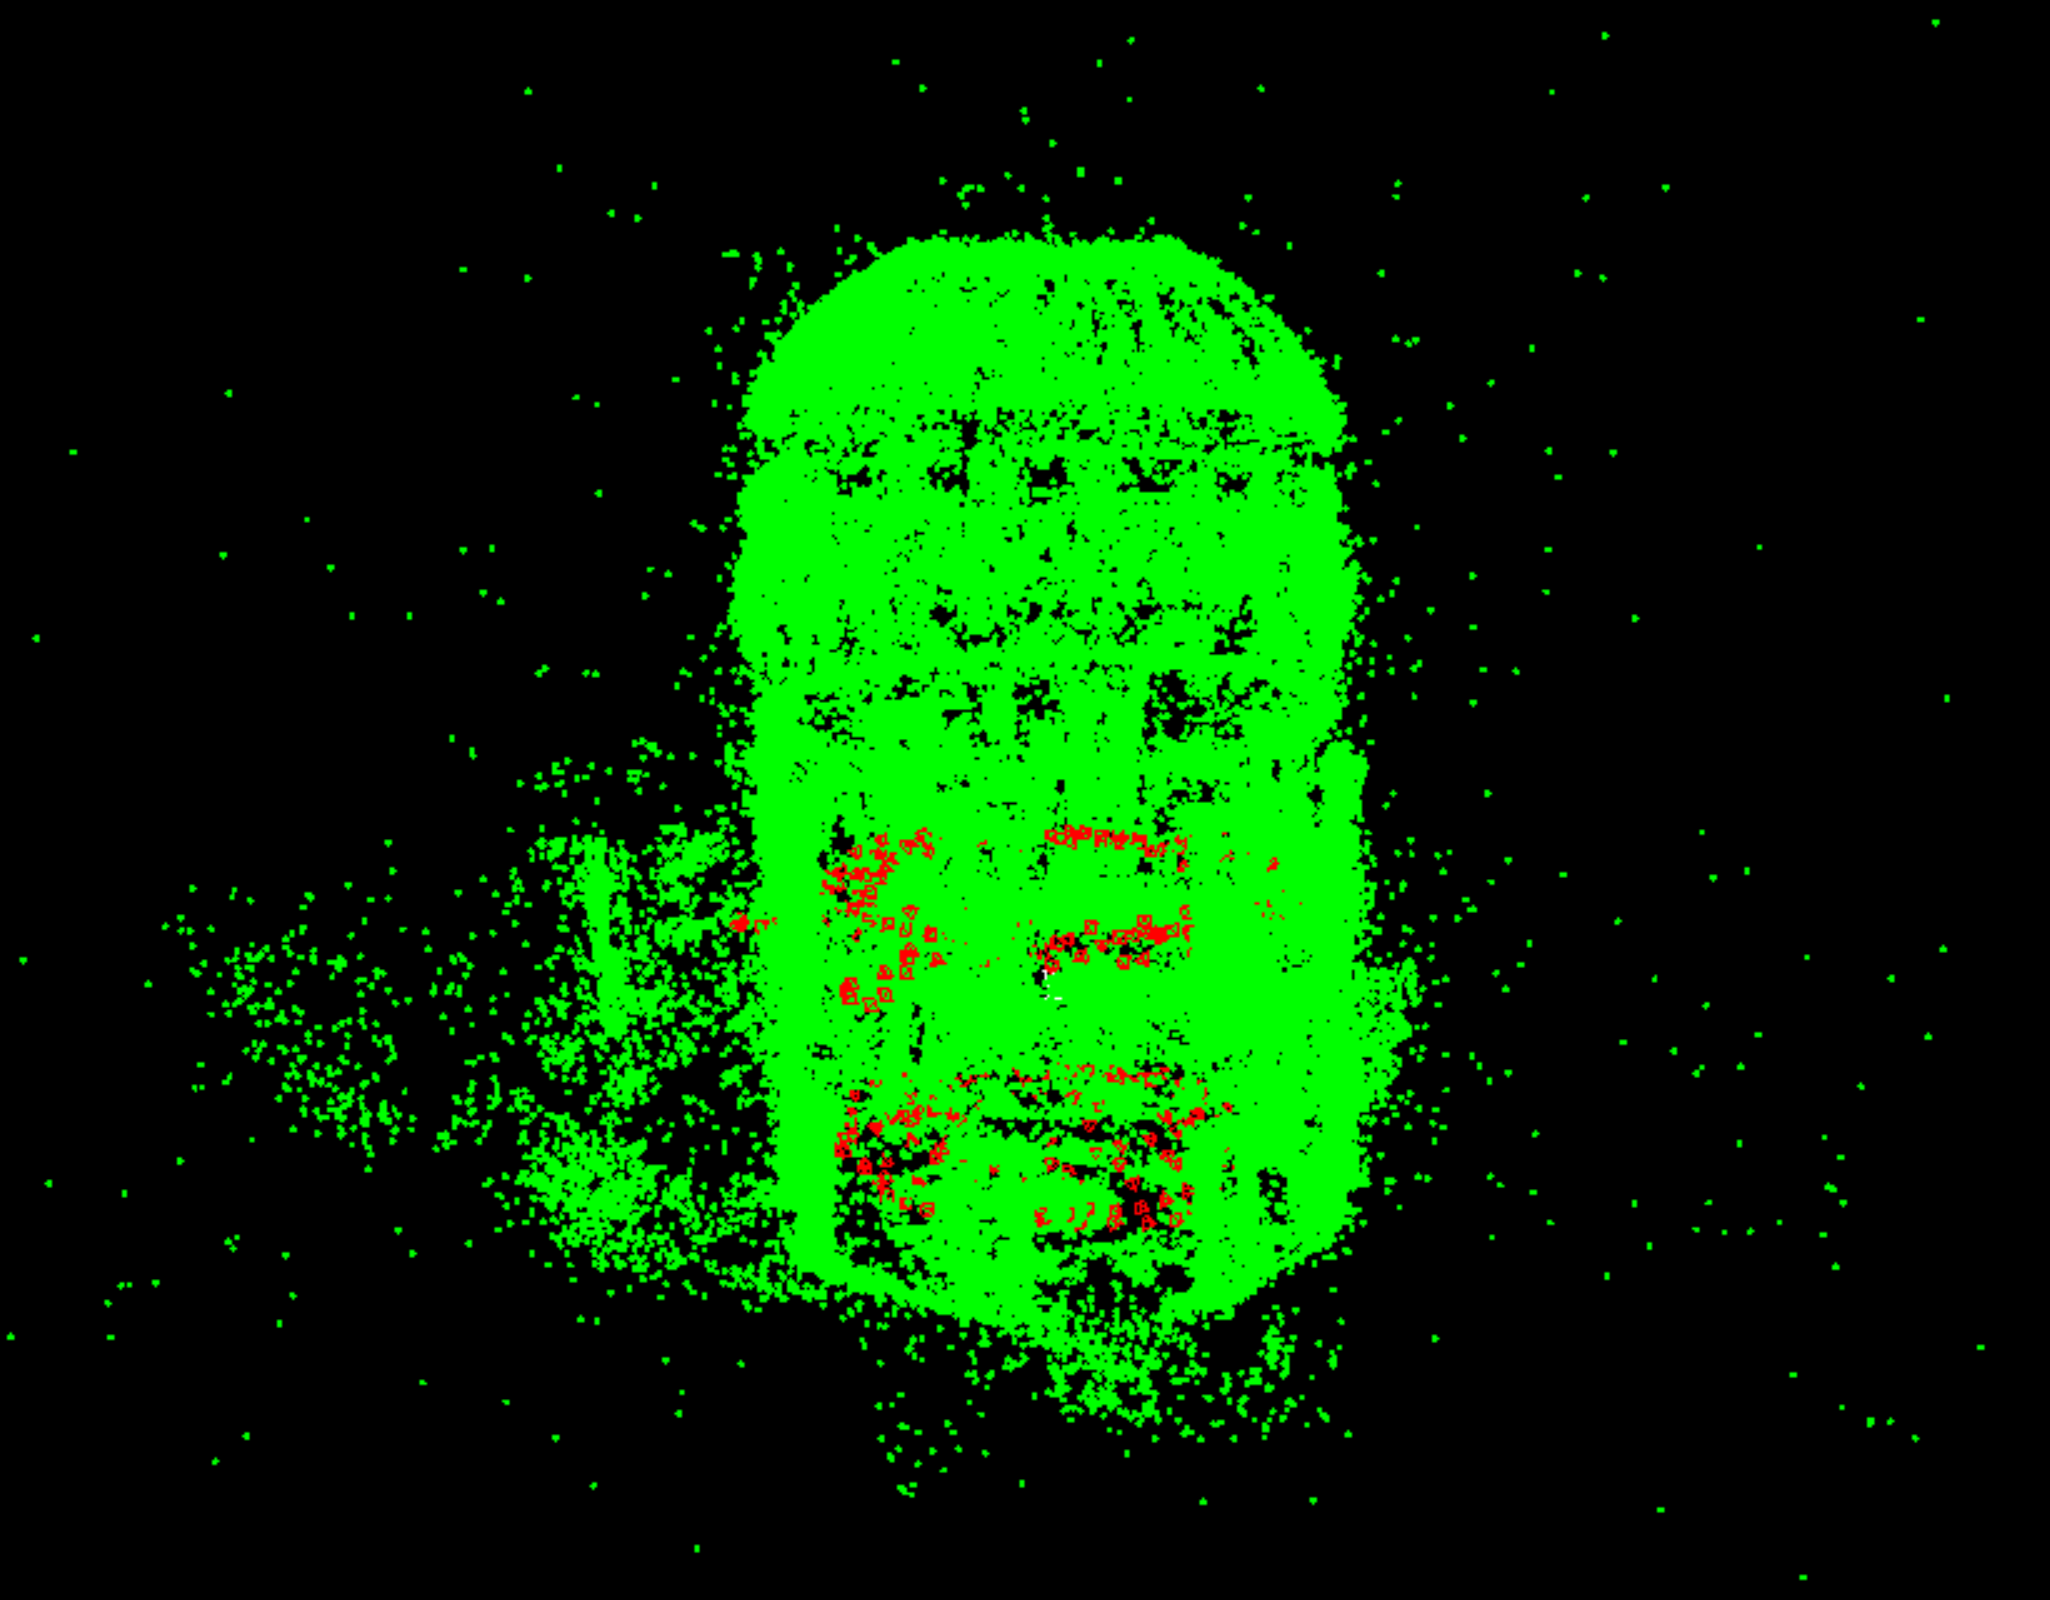
\includegraphics[width=\linewidth]{datas/helper/test_pointcloud_museum.png}
    \end{subfigure}

    \caption{Résultats des tests pour le dataset Museum}
    \label{fig:test_museum}
\end{figure}

\end{document}


